\chapter{Diode cell}
\label{cha:diode}
\section{Introduction}
As has been seen in both Chapter \ref{cha:45} and Chapter \ref{cha:splay_uniform}, interesting and unique director profiles can be observed when a nematic liquid crystal is made to flow through the application of a pressure gradient. Under this flow, the director's reorientation is greatly influenced by the bounding layers and the alignment conditions prescribed through the cell fabrication.

As was hinted at in Chapter \ref{cha:pretilt} (where two separate recipes were used to promote large pretilt angles of the director at the cell walls), this chapter goes on to look at an interesting idea for an extremely novel flow cell design, whereby the nematic liquid crystal \textit{itself} is made to respond to flow like a valve or diode. The idea is that the flow cell exhibits a preferential flow direction, dictated by an asymmetry in the pressure head required to achieve the same volumetric rate in both directions through the flow channel. 

In this case, this is experimentally attempted by fabricating a flow cell in which a large pretilt angle with a splayed geometry is created and aligned parallel to the flow direction.

\subsection{The idea}
The impetus behind this experiment came from a conversation on flow channels where the question was posed, \textit{`If a circular flow channel filled with a liquid crystal had a preferential flow direction, could the liquid crystal be made to flow in that direction through thermal fluctuations`kicking' the molecules into action?'}

The idea is perhaps best demonstrated in Figure \ref{fig:schematic_diode}, whereby one can intuitively imagine that in order to achieve the same volumetric flow rate in both the `easy' direction (green arrow) and `hard' direction (red arrow) through this channel via the application of a pressure gradient, a larger pressure gradient will be required in the `hard' direction. This `feels' correct as it is already known that for flow in the `easy' direction, the director will reorient to achieve the Leslie angle of opposite sign in the top and bottom halves of the cell, but what will happen when flow is constrained to be in the `hard' direction? Here, it also seems intuitive that the director will attempt to bend back on itself to create a complex and highly distorted director profile (with the gradients in $\bm{n}$ changing rapidly), forcing more of the liquid crystal to be in the vertical state, having a higher viscosity.

This chapter will now go on to look at the experiments undertaken to try to measure any difference in the pressure gradient required across a cell fabricated with a similar director geometry as is schematically shown in Figure \ref{fig:schematic_diode} in order to achieve the same volumetric flow rate in both directions. This experimental section is followed by a short section regarding the attempted simulation of such a cell, followed by a look at how the experiment could be extended and improved upon.

\begin{figure}
\begin{center}
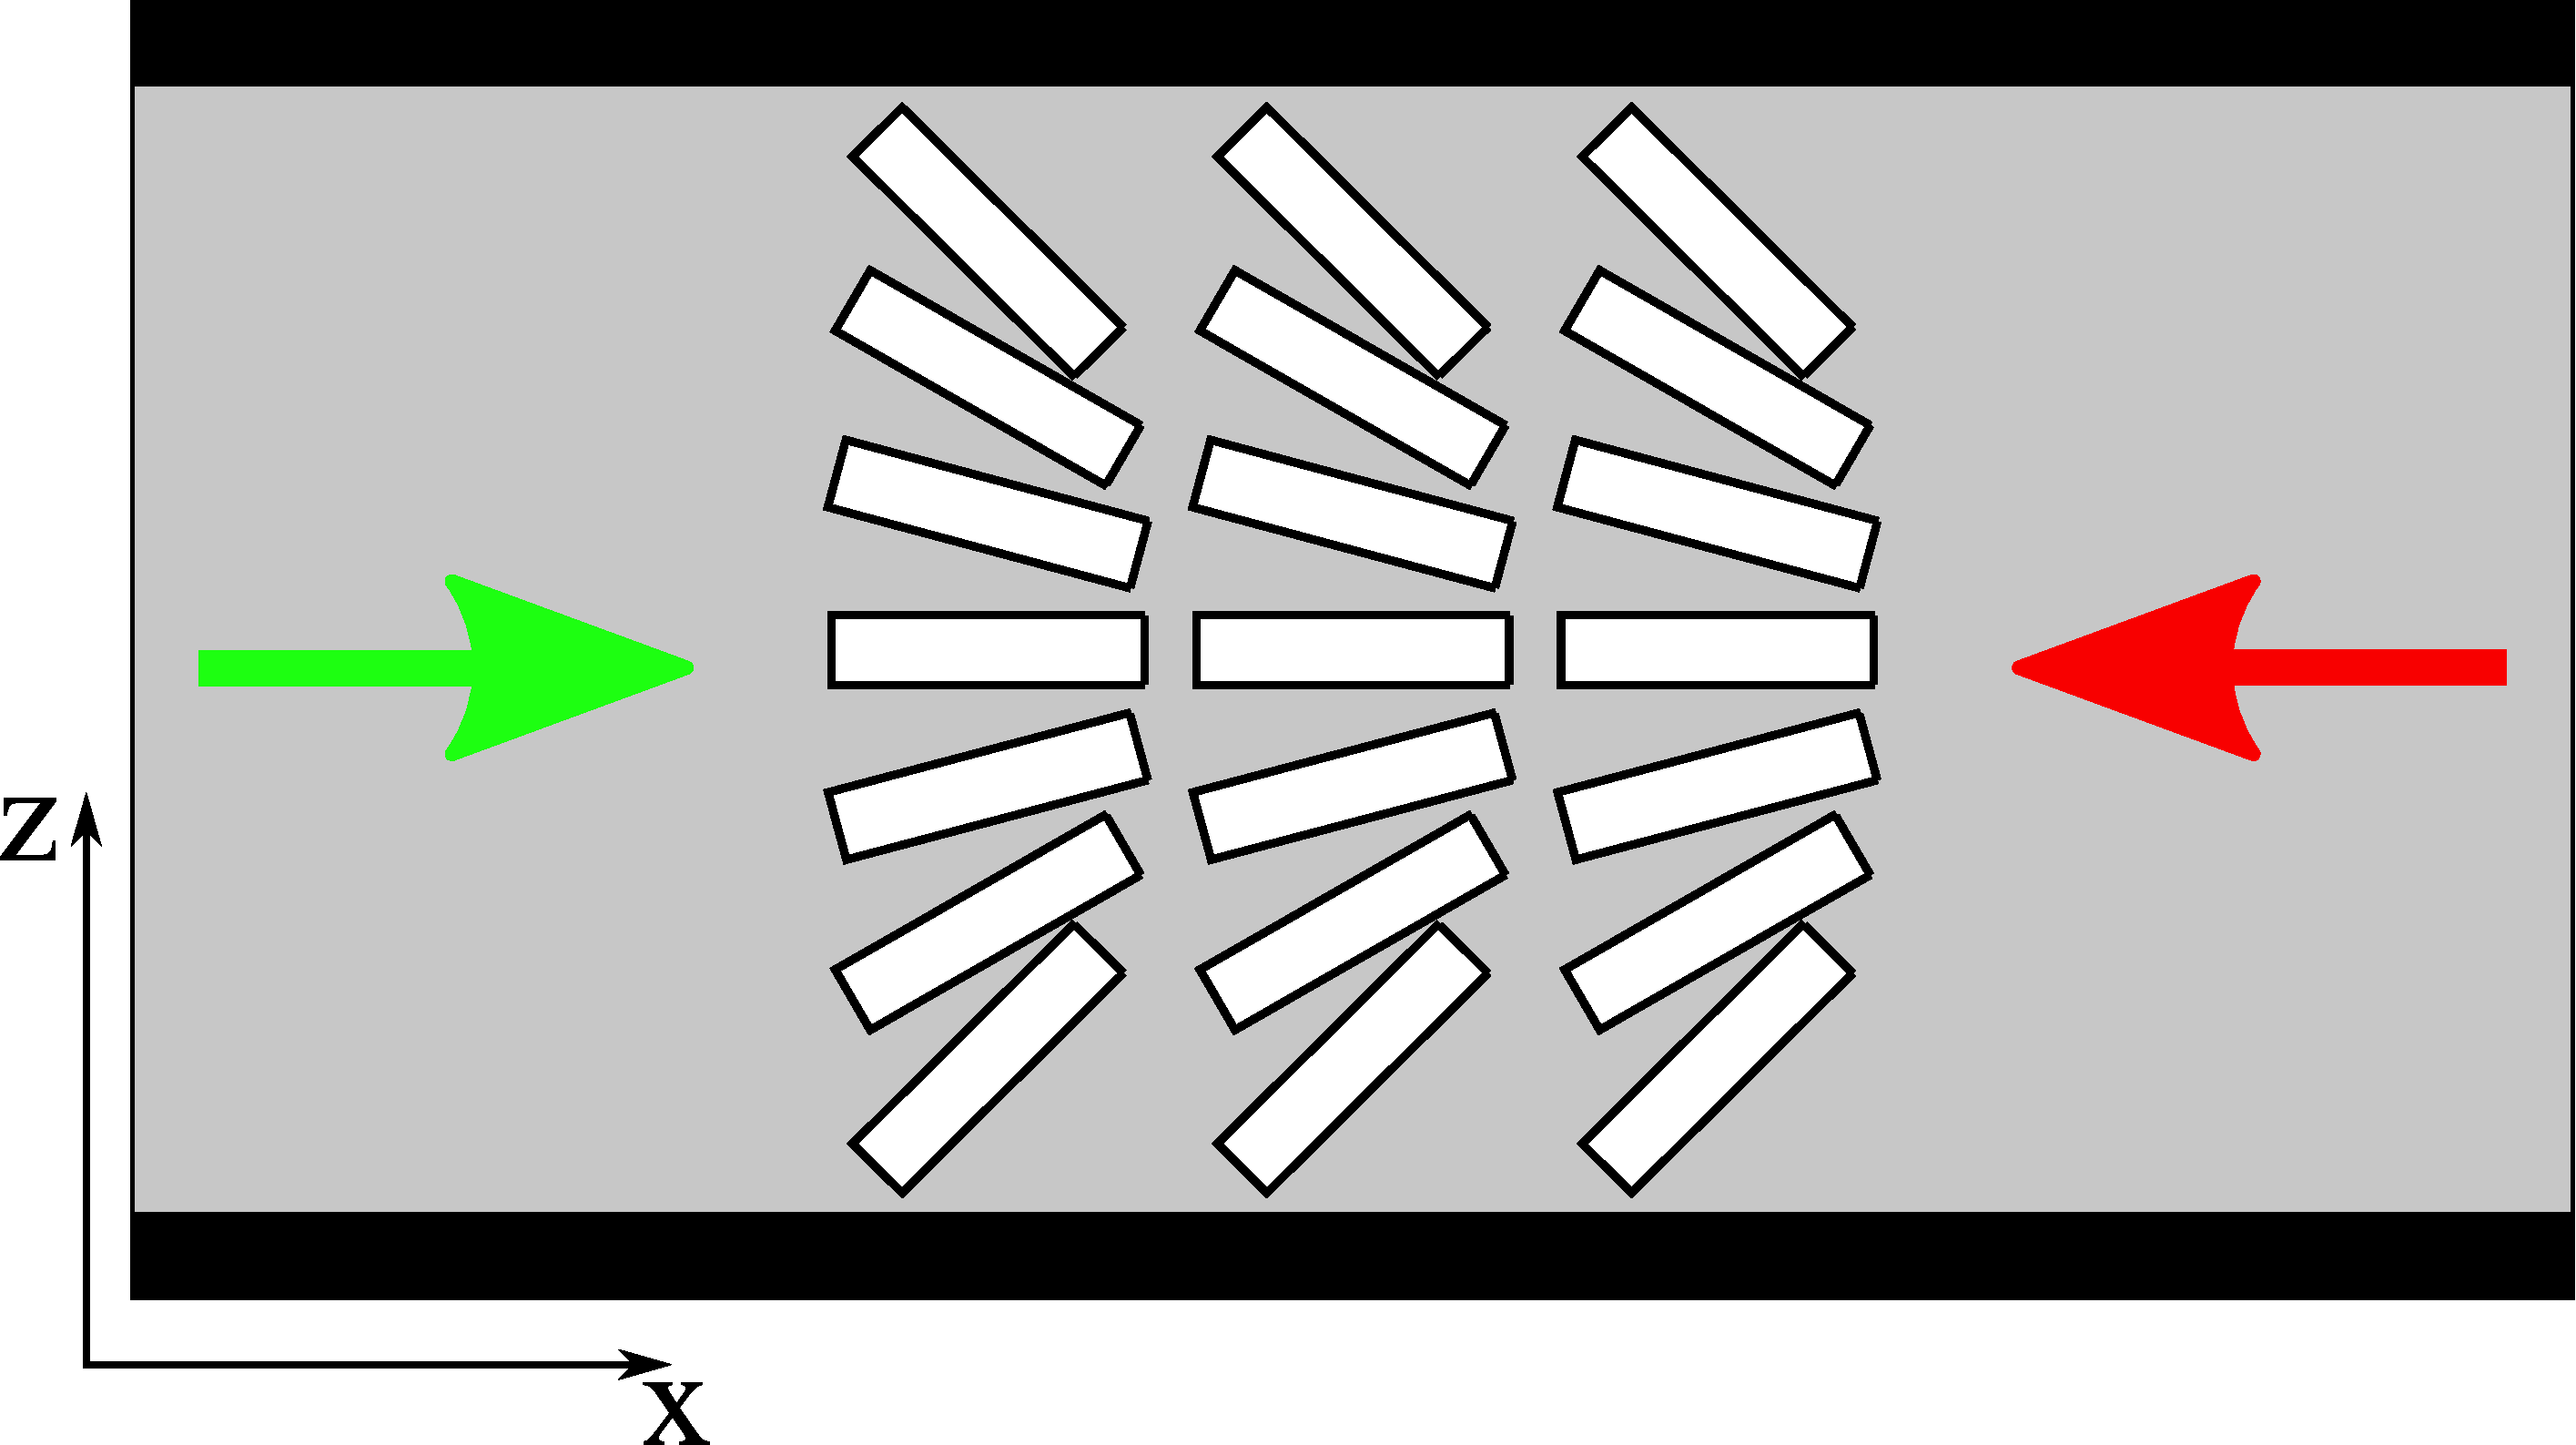
\includegraphics[width=0.7\textwidth]{Figures/Diode/schematic_diode}
\end{center}
\caption[Schematic diagram of a splayed `diode' cell]{\label{fig:schematic_diode}Schematic diagram of the idea behind the diode cell behaviour. A splayed geometry is depicted with flow directions indicated as being `easy' (the green arrow) and `hard' (the red arrow). In this case, the director is azimuthally aligned to be parallel to the flow direction.}
\end{figure}

\section{Experimental setup}
\label{sec:experimental_deets}
In order to physically observe the pressure gradient across the cell, an experimental method had to be developed that would allow for the pressure head at both ends of the cell to be measured whilst not inhibiting the connection to the syringe pump. It was decided that the best way to do this would be to introduce two extra holes to the cell at either end of the flow channel, in order to attach two more tubes (rising vertically) allowing for measurement of the height that the liquid crystal would reach due to the flow. Essentially, this turns the cell and tubing into a conventional manometer. The next sections go on to describe the experimental apparatus designed and built to achieve this aim.

\subsection{Cell clamp}
Figure \ref{fig:case} shows photographs of the diode cell in a bespoke clamp made for this experiment. The two aluminium plates of the clamp are screwed together with ten screws, allowing for an even pressure to be applied across the whole of the glass cell walls.\footnote{A viewing window is milled out of both sides of the clamp to allow for optical probing of the cell under flow should it be required.} Two smaller manometer holes are also drilled into the top glass plate (see Figure \ref{fig:case}(a)), just inside the main inlet and outlet holes of the cell. These two holes form the means of measuring the pressure gradient across the cell.\footnote{Where the manometer tubes meet the cell, the brass connectors are bent through 90$^{\circ}$ so as to point vertically upwards.} Polypropylene hose is attached and fed directly upwards through another bespoke piece of apparatus which holds the manometer tubes at a set distance apart, against a ruler (for measuring column height) as shown in Figure \ref{fig:case}(b).

\begin{figure}
\begin{center}
\subfigure[Cell clamp]{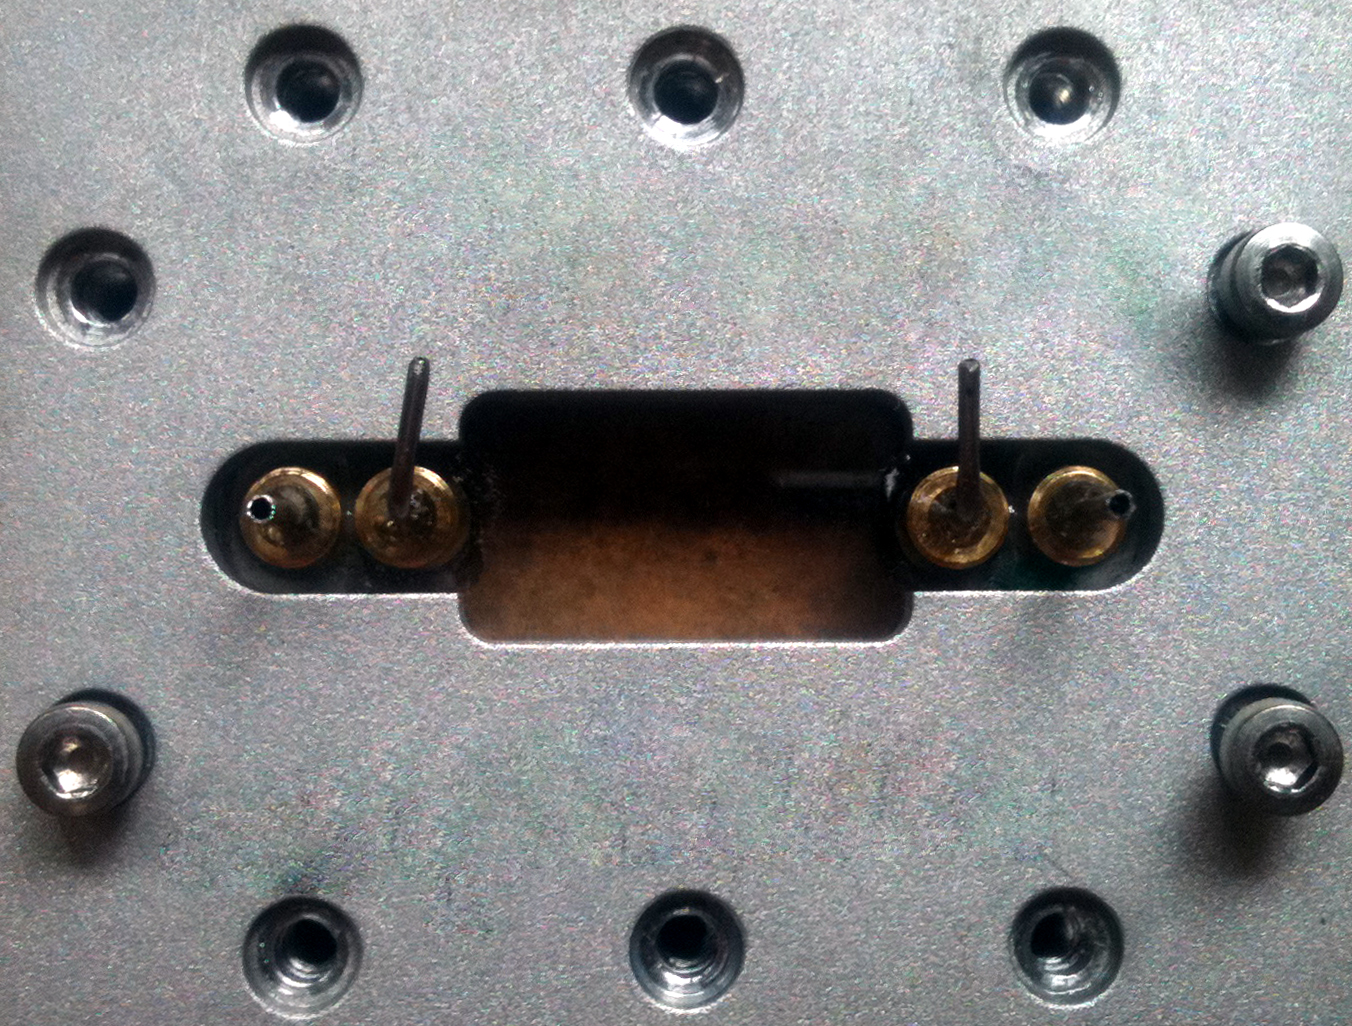
\includegraphics[width=0.5\textwidth]{Figures/Diode/case}}\\
\subfigure[Cell clamp and manometer tubing]{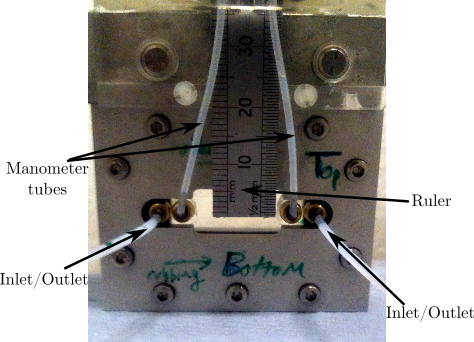
\includegraphics[width=0.7\textwidth]{Figures/Diode/case_cell_annotated}}
\end{center}
\caption[Aluminium cell clamp]{\label{fig:case}(a) Aluminium cell clamp. The flow cell is sandwiched between the two aluminium plates with a viewing window milled out of the centre. (b) The aluminium cell clamp in the experimental setup, with plastic tubing creating a manometer for measuring the pressure difference across the length of the cell. Plastic tubing is also used for the inlet and outlet of the cell which are connected to the inlet and outlet of the flow-switch shown in Figure \ref{fig:valve_states}.}
\end{figure}

In principle, the apparatus in Figure \ref{fig:case} alone could be used to make a measurement of the pressure gradient across the cell when flown at a constant volumetric flow rate in both directions. However, after many months of trying to get this system to work, it was decided that a better way of enabling the flow of the liquid crystal in both directions was needed. This decision was made as it was found that when removing the syringe pump from one end of the device and attaching it to the other (in order to flow the liquid crystal in the opposite direction), air bubbles would almost always be introduced into the flow cell and surrounding tubing, as well as increasing the mechanical stress on the inlet and outlet connections, which often resulted in failing seals and repetitive leaking of liquid crystal at the cell.

\subsection{Valve}
Figure \ref{fig:valve_states} shows a schematic diagram of the solution to this problem, whereby a valve having six connections (which can be switched between two operational states) was introduced. These two operational states of the valve can be seen in Figures \ref{fig:valve_states} (a) and (b) respectively. In switching the valve from the first state to the second state, the direction of flow in the cell can be reversed, importantly, \textit{with no need to disconnect the syringe pump} or to change the outlet pipe of the whole system. This is shown in Figure \ref{fig:valve_states}, whereby switching the valve between the two states results in the internal connections (green arrows) shifting and producing flow in the reversed direction in the cell (shown by the blue arrows in the schematic diagram above the photo of the valve in (a) and (b)). Crucially, in both states the inlet and the outlet \textit{to the valve} remain unchanged, meaning that there is no need to disconnect the syringe pump or disrupt the system in any way. The addition of the valve leads to a far more stable experimental setup, whereby the direction of flow in the cell can be changed quickly and easily\footnote{It should be noted that as six new connections have also been introduced to the system, this adds more possible sites for leakage or poor connections. This could easily lead to erroneous pressure measurements.}. 

\begin{figure}
\begin{center}
\subfigure[Left to Right]{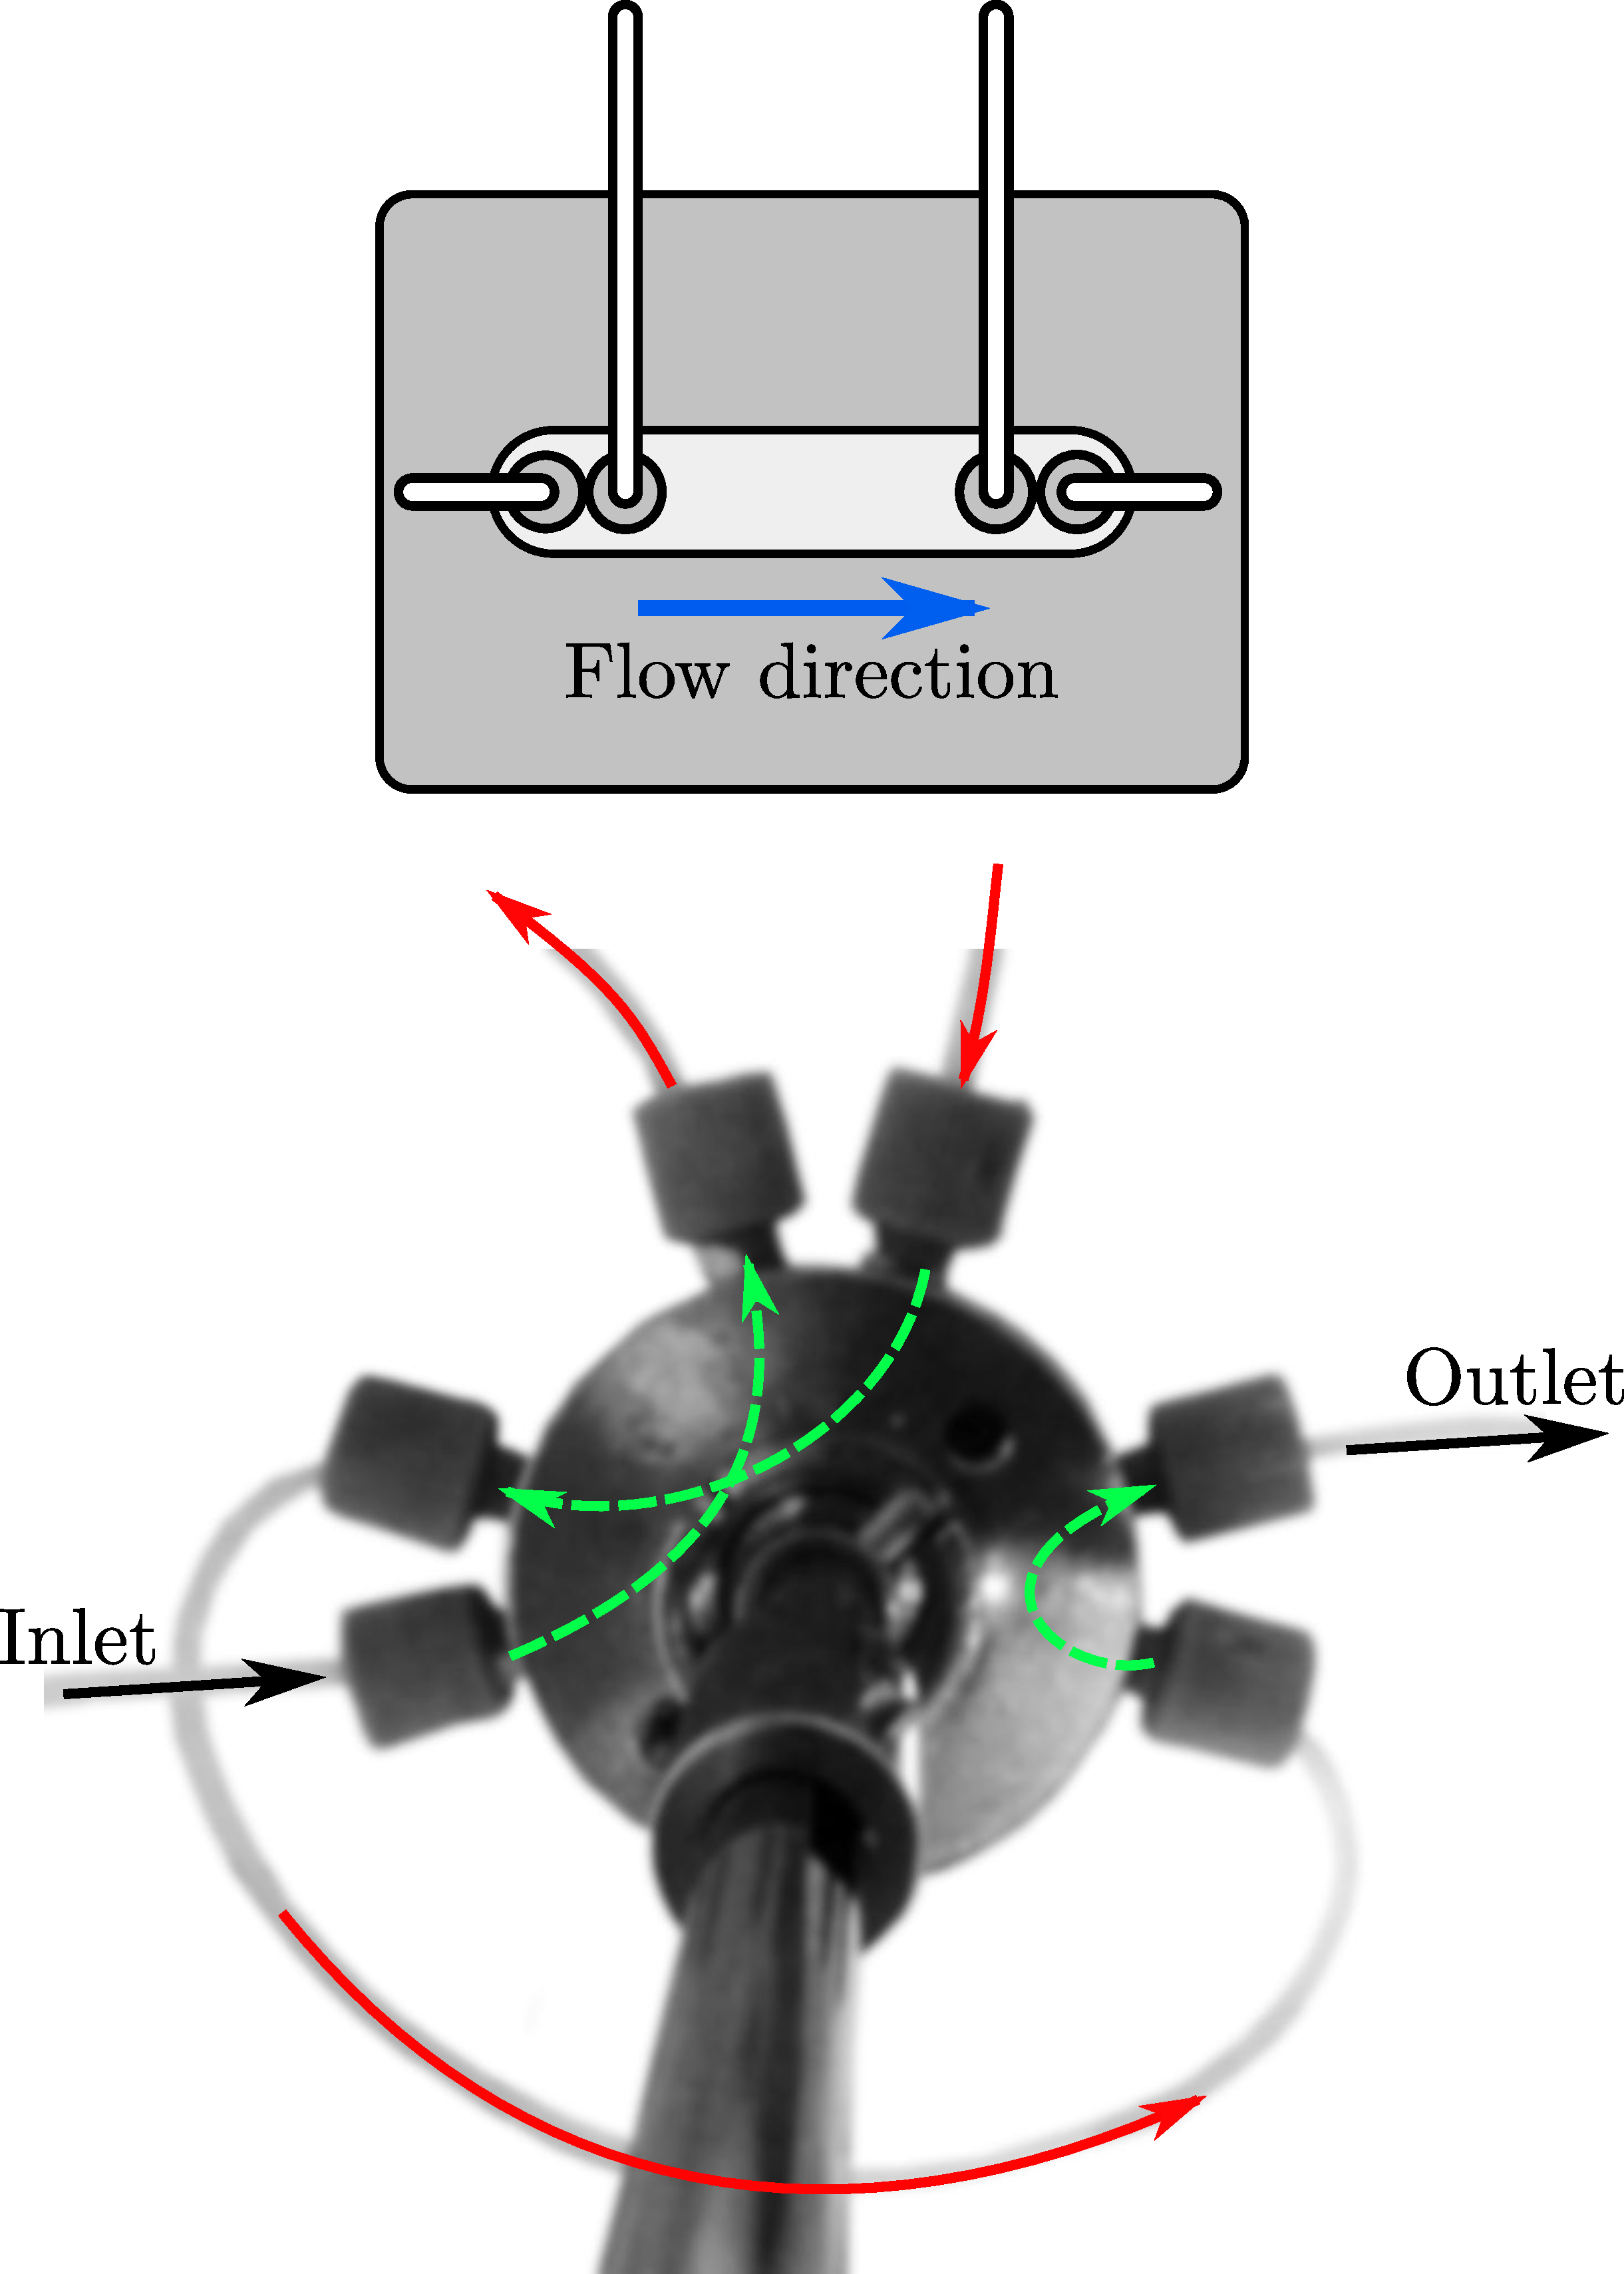
\includegraphics[width=0.48\textwidth]{Figures/Diode/valve1pdf}}
\subfigure[Right to Left]{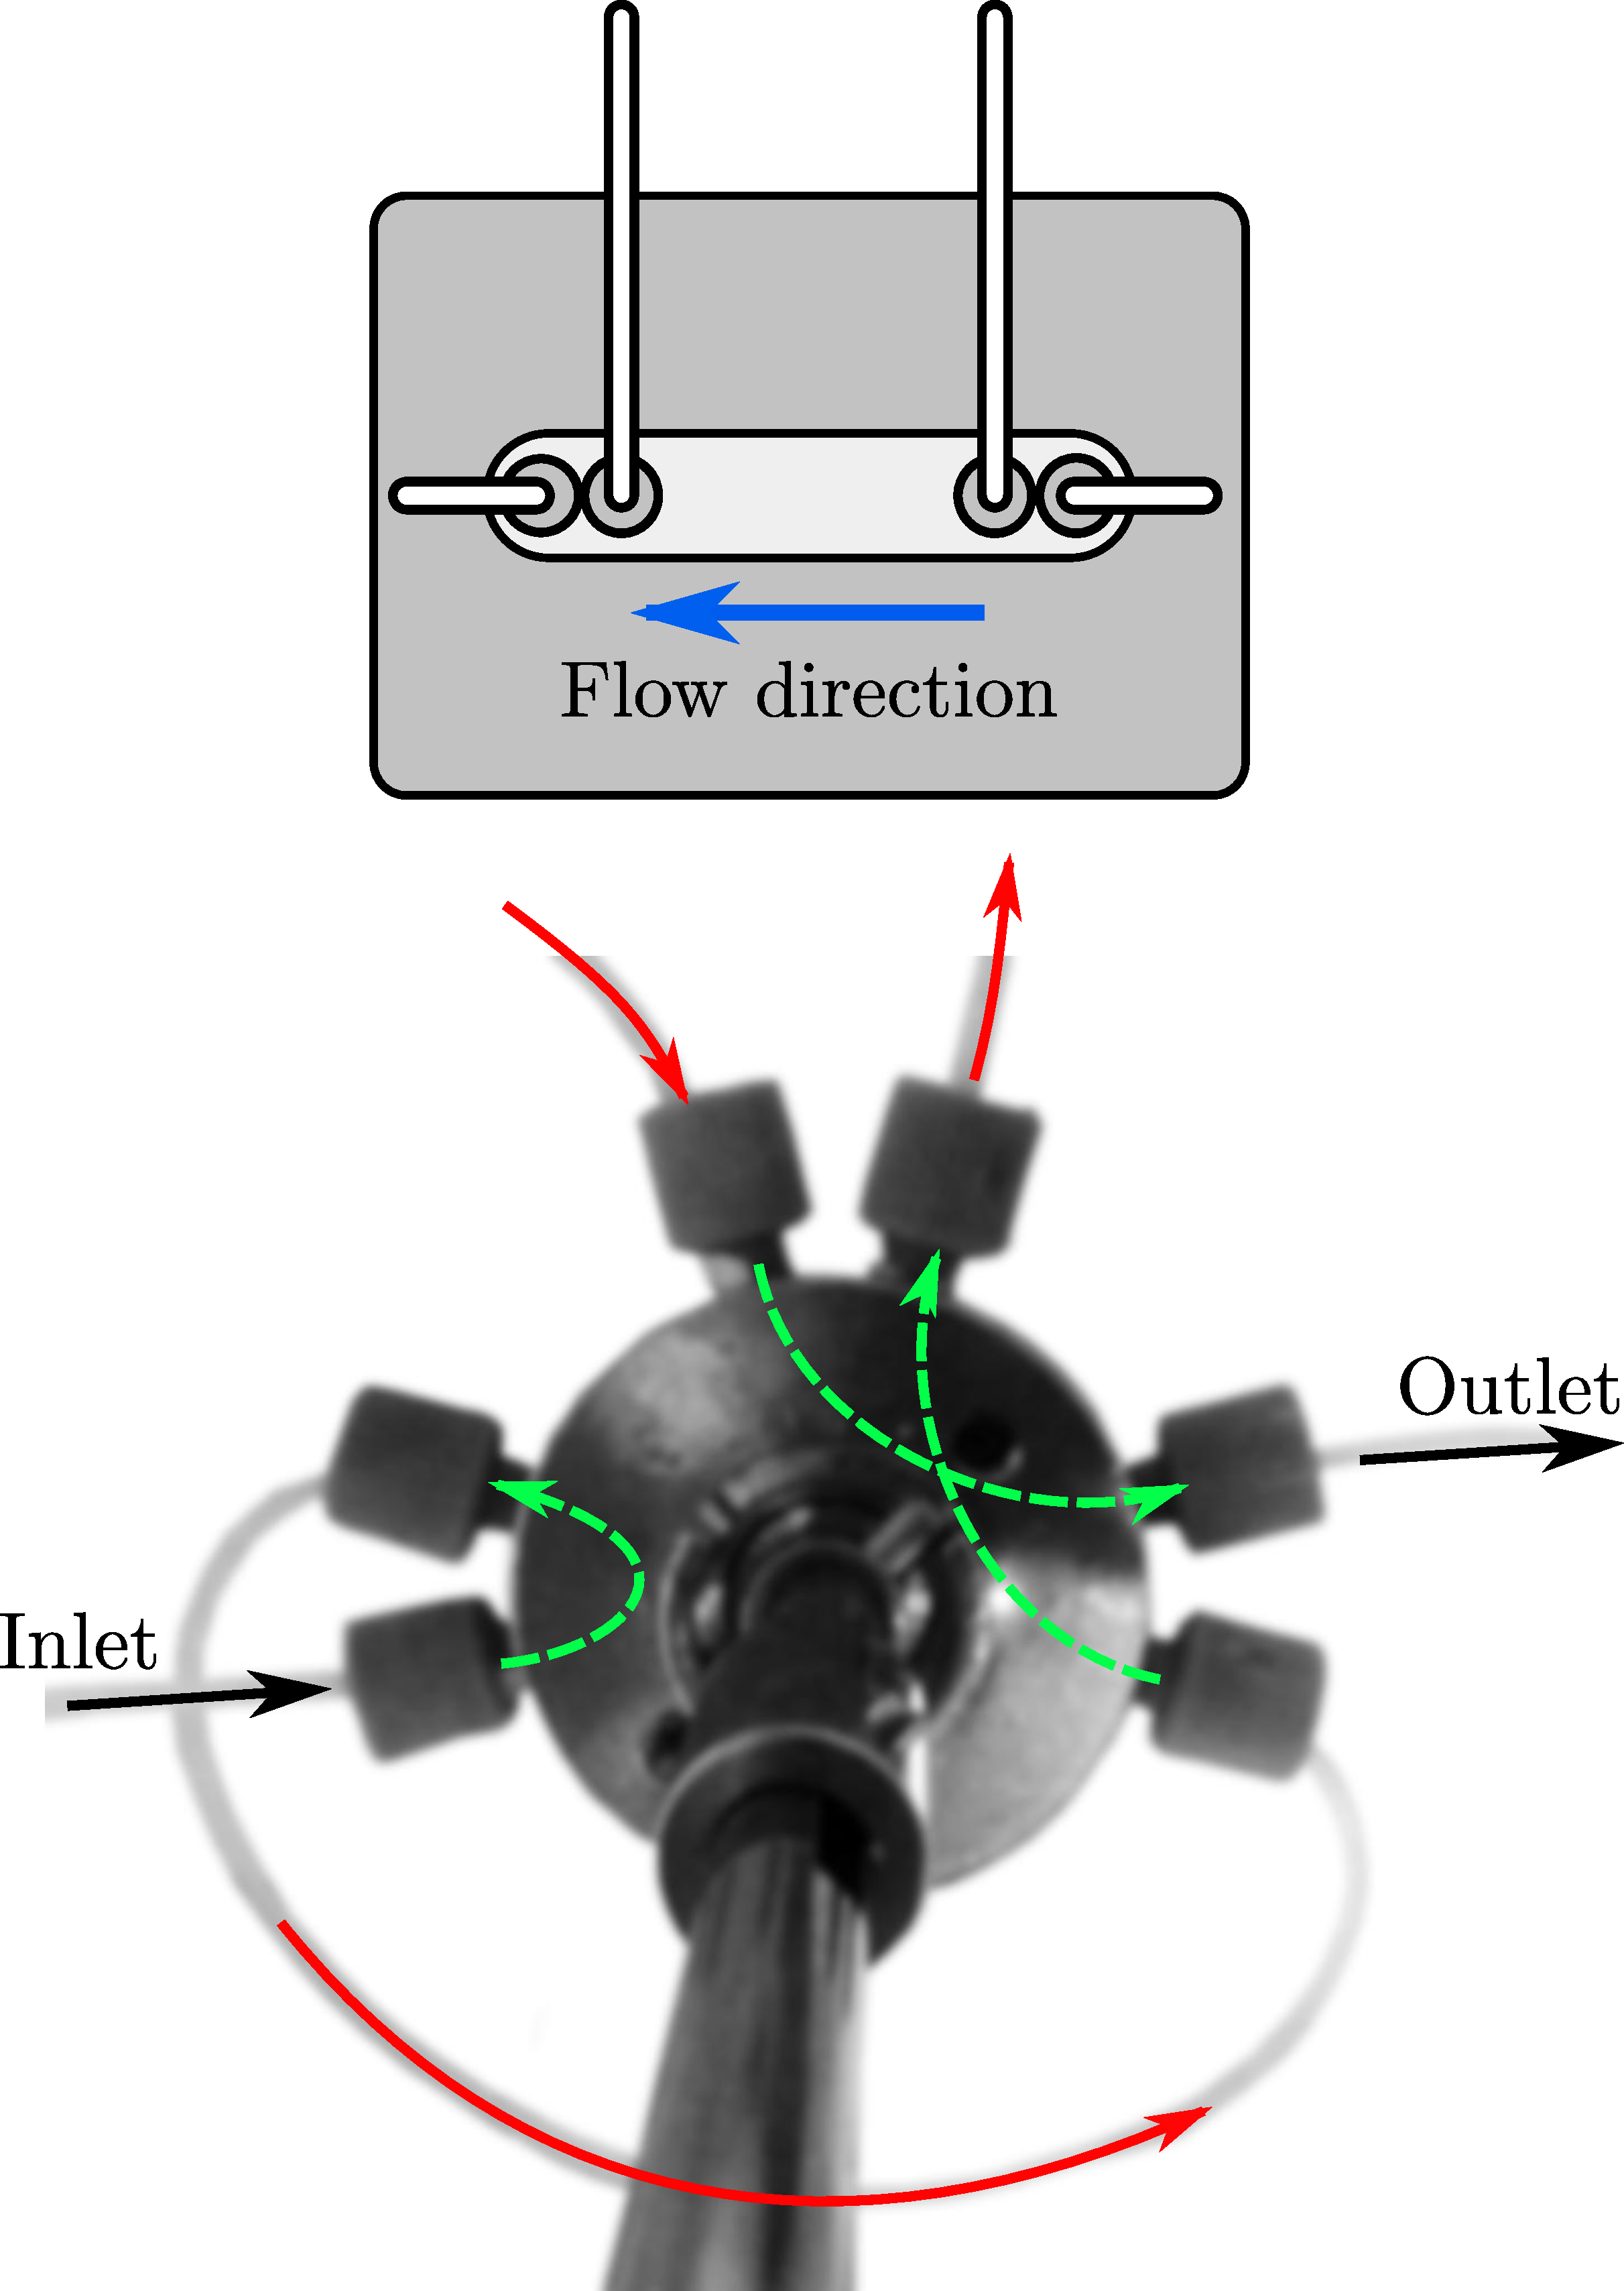
\includegraphics[width=0.48\textwidth]{Figures/Diode/valve2pdf}}
\end{center}
\caption[Workings of two state valve]{\label{fig:valve_states}(a) The valve in the first \textit{left-to-right} state. (b) The valve in the second \textit{right-to-left} state. The green dashed arrows denote the inner connections of the valve, the red arrows denote the external connections made with plastic tubing, the black arrows denote the inlet/outlet connections and the blue arrow shows the direction of flow in the cell. The important function of the valve is that the inlet and outlet connections do not change position when the valve is switched between the two states, meaning that the liquid crystal can be flown in both directions without removing the cell from the setup.}
\end{figure}

\subsection{Polystyrene housing}
Ultimately, to test whether there is any valve-like behaviour from the large pretilt angle and splay geometry in the cell (and also to rule out any valve-like behaviour caused by the experimental set up), it is required that the cell is heated to the isotropic phase. Once in this state (no longer liquid crystalline), there should be no asymmetry in the pressure difference needed for a fixed volumetric flow rate to flow in either direction, i.e. no valve-like behaviour (much like one would expect to see if flowing water through the cell). In order to achieve this, the whole system must be heated to the isotropic phase so that there is no phase boundary at any point within the setup. This means that a housing had to be designed and built to enclose the cell, the valve, the syringe pump and the outlet reservoir whilst maintaining all components at an elevated temperature and allowing for physical reading of the liquid crystal column heights.

Figure \ref{fig:heat_box_perspective} shows a schematic diagram of the final design of the housing. Approximately two inch thick polystyrene walls form an enclosure around the equipment, with a large copper base plate placed on the  bottom surface of the box. Copper tubing connected to a hot water bath (maintained at a given temperature) is then connected (ensuring a good thermal contact) and snaked along the underside of the copper base plate within the housing. This allows for water of a given temperature to be circulated through the tubing, raising the temperature of the copper base plate and ultimately the air within the enclosure.

\begin{figure}
\begin{center}
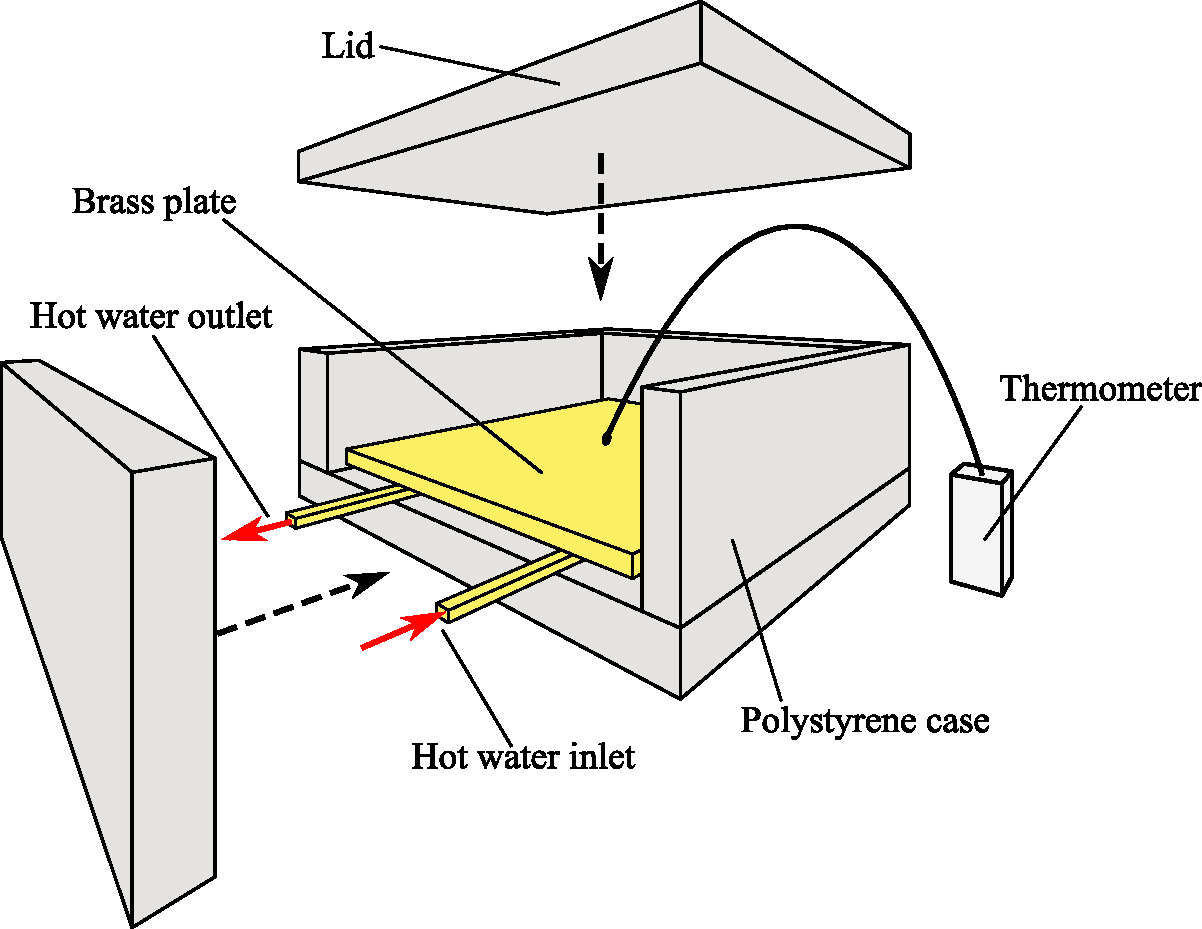
\includegraphics[width=0.8\textwidth]{Figures/Diode/heat_box_perspective}
\end{center}
\caption[Schematic diagram of housing for temperature controlled experiment]{\label{fig:heat_box_perspective}Schematic of the polystyrene housing used to enclose the experimental equipment. Approximately 2 inch thick polystyrene walls house the syringe pump, flow-switch, cell and manometer tubing/rig. The brass plate at the bottom of the enclosure has brass tubing coiled underneath it, through which hot water is passed from a hot water bath. A remote thermocouple is used to measure the air temperature inside the enclosure.}
\end{figure}

Figure \ref{fig:heat_box_perspective} also shows the thermocouple which was used to measure the temperature of the cell in the enclosure\footnote{A standard mercury thermometer was also used to monitor the temperature of the hot water bath.}. Figure \ref{fig:heat_box_photos} shows two photographs of the experiment in the housing both open (a) and closed (b). Figure \ref{fig:heat_box_photos} (a) shows the syringe pump, cell and valve within the housing. A small extra enclosure was designed and added to the top of the housing to allow for the manometer tubes to project above the lid of the housing. This small extra enclosure has a lid on a hinge, allowing for reading of the column heights against the ruler without having to open the main enclosure and alter the temperature of the experiment.

\begin{figure}
\begin{center}
\subfigure[]{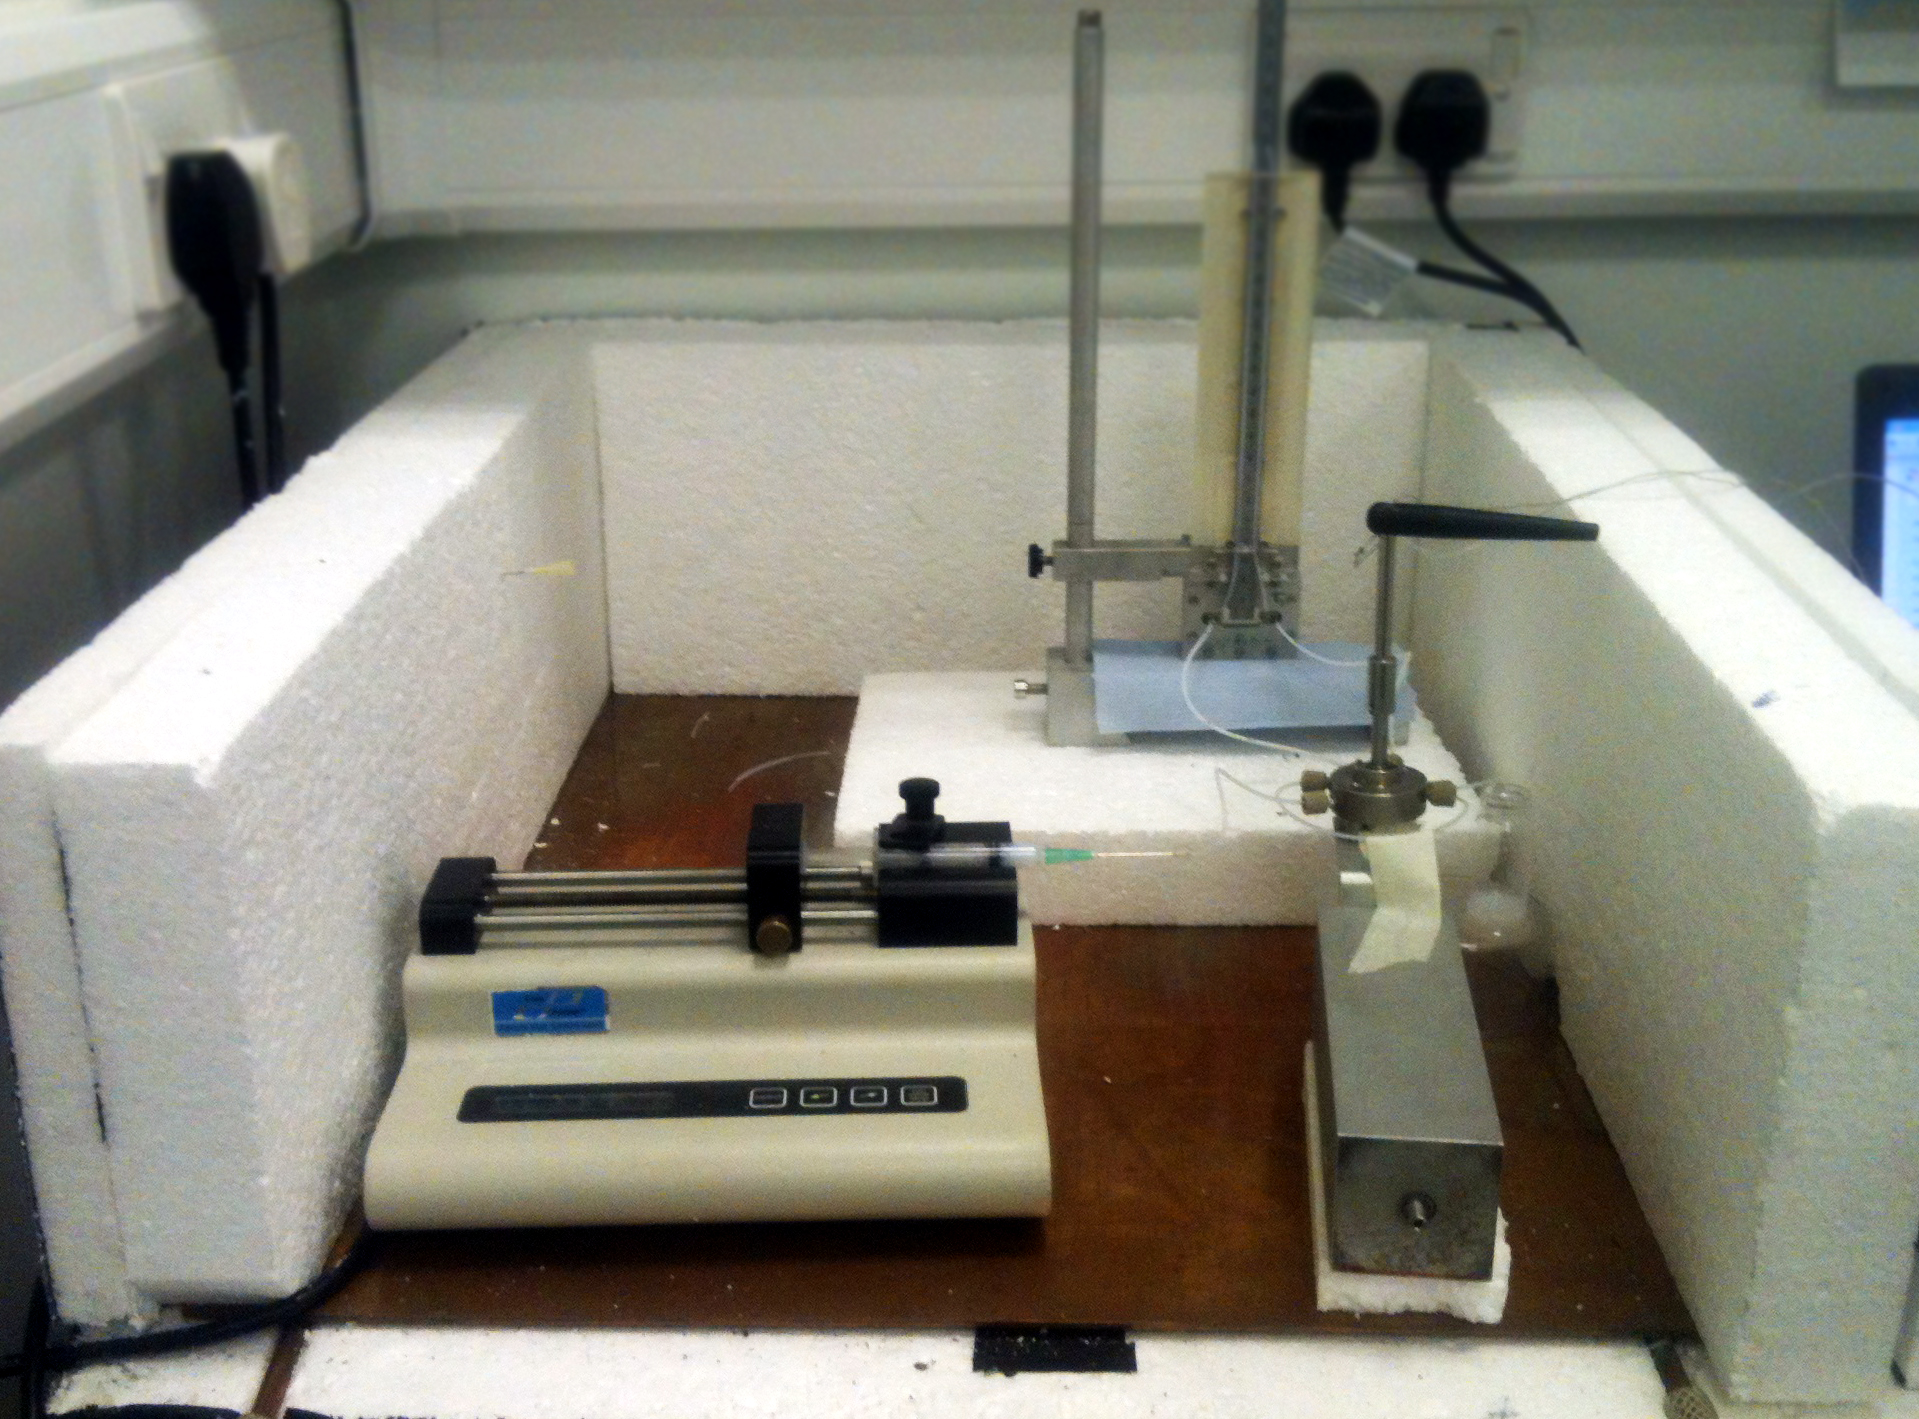
\includegraphics[width=0.6\textwidth]{Figures/Diode/open_box}}
\subfigure[]{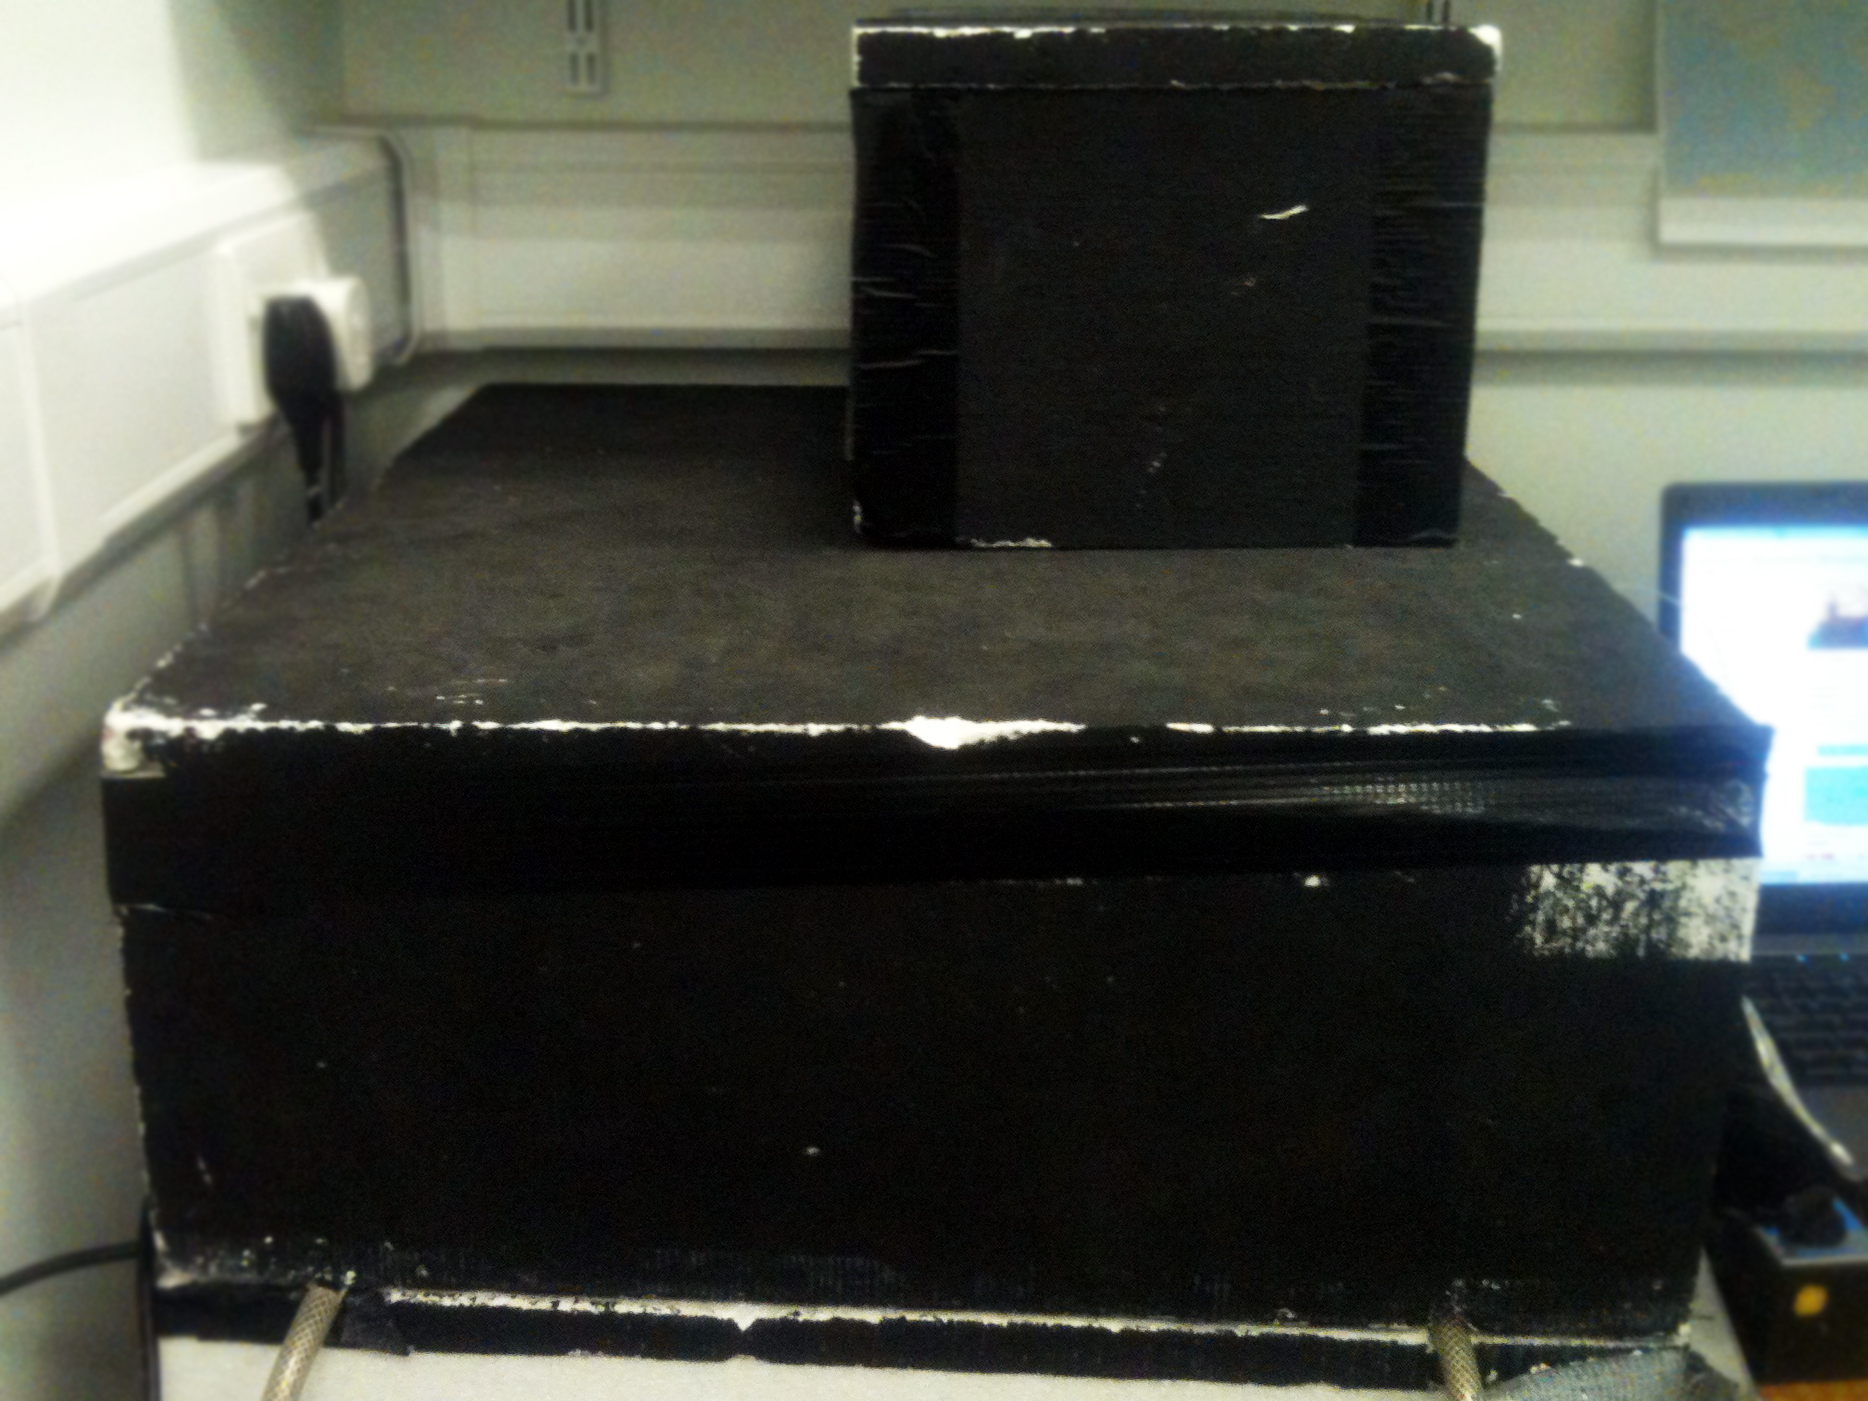
\includegraphics[width=0.6\textwidth]{Figures/Diode/closed_box}}
\end{center}
\caption[Pictures of polystyrene housing for isotropic phase experiments]{\label{fig:heat_box_photos}(a) A photograph of the polystyrene enclosure used to house the experimental equipment. The copper plate at the bottom of the box can clearly be seen. (b) Shows the polystyrene enclosure in the closed state. An extra polystyrene box is added to the top of the main enclosure in order to keep the manometer tubing within the enclosure.}
\end{figure}

\subsection{Data acquisition}
The basic procedure employed here for measuring the pressure gradient across the length of the cell and determining whether or not the liquid crystal behaves likes a valve, is achieved by first setting a constant volumetric flow rate at the syringe pump in one direction through the cell. After a given time, the liquid crystal will have flowed up the two vertical manometer tubes at both ends of the cell to a height $h$ defined by

\begin{equation}
P=\rho gh
\end{equation}

\noindent where $P$ is the pressure in the liquid crystal causing the flow at that point, $\rho$ is the density of the liquid crystal and $g$ is acceleration due to gravity $\left(g\approx9.8 \text{ m/s$^2$}\right)$. By measuring the value of $h$ in both columns (which will be different ($h_{1,2}$)), the pressure gradient across the length of the cell can be calculated through the change in pressure,

\begin{equation}
\Delta P=\left(P_1-P_2\right)=\rho g \left(h_1-h_2\right)
\label{eq:pressures}
\end{equation}

In order to acquire data to make this calculation, the column heights (the height that the liquid crystal reaches in the manometer tube) of the left and right manometer tubes are recorded as a function of time, commencing from when the flow is first switched on. The resulting curves allow the point at which the column height has achieved its equilibrium state to be identified, namely when the value of the column height is invariant with time. Once the liquid crystal had reached it's equilibrium height within the manometer tubing, the valve can be switched so that the liquid crystal now flows in the opposite direction through the cell at the same volumetric flow rate.

This process needs to be carried out over a range of flow rates in both directions through the cell, and if done completely, a comparison of the pressure gradient required to achieve the same volumetric flow rate in both directions through the cell can be made. As stated earlier, for an isotropic liquid, there should be no difference in the pressure head needed to achieve the same constant volumetric flow rate in both directions, whereas, for a liquid crystal under the right initial alignment conditions, this may not be the case.



\section{Results}
What follows are the results from a series of experiments from a range of cells. The results section has been split into three sub sections. These sections are entitled `First diode behaviour' (\ref{sec:first_diode}), `Second diode behaviour' (\ref{sec:second_diode}) and `Isotropic phase' (\ref{sec:isotropic}).

`First diode behaviour' refers to the first constructed cell to show valve-like behaviour. `Second diode behaviour' refers to a second cell constructed which again showed valve-like behaviour. `Isotropic phase' refers to the experiment in which the second cell to exhibit valve-like behaviour was heated to the isotropic phase to examine the effects of phase change upon diode properties.


\subsection{First diode behaviour}
\label{sec:first_diode}
A cell was fabricated using the over-baked Nissan SE-1211 recipe described in Chapter \ref{cha:pretilt}. Here, the glass plates were rubbed parallel to the long side of the slide (the flow direction) at a rubbing parameter value of 4.2 at the HP Labs rubbing machine in order to achieve a pretilt angle of approximately 45$^{\circ}$ on glass as shown by Figure \ref{fig:ito_glass}. The slides were then fabricated into a parallel aligned cell in order to create a splayed director geometry. This cell was then placed into the aluminium cell clamp and set up as shown in the polystyrene enclosure for pressure measurements. For all data in this chapter, left to right is considered the `easy' direction and `right to left' is considered the `hard' direction.

A series of preliminary experiments were carried out to fully characterise the response of the cell and also eliminate the possibility that if any diode behaviour were to be observed, that it was not a result of the experimental set up. For example, it was questioned as to whether or not kinks, bends and stresses on the network of tubing connecting the valve to the cell could have an asymmetric effect on the column heights and pressure gradient measured, or whether perhaps if the cell were to be positioned lower than the valve, or if the main outlet to the whole system was moved, would the same pressure heads still be measured? A selection of the graphs from these experiments are shown in Figure \ref{fig:first_diode_small_graphs} (a) to (d). Column heights are plotted here as a function of flow rate and time since the flow was started. Here, rather than filling the cell to the highest flow rate and only backing off the flow rate to the lowest value, the flow rate is lowered and increased during the same data set to see how the column heights achieve their equilibrium values.

\begin{figure}
\begin{center}
\subfigure[]{\includegraphics[width=0.49\textwidth]{Figures/Diode/first_diode/small_graphs1}}
\subfigure[]{\includegraphics[width=0.49\textwidth]{Figures/Diode/first_diode/small_graphs2}}
\subfigure[]{\includegraphics[width=0.49\textwidth]{Figures/Diode/first_diode/small_graphs3}}
\subfigure[]{\includegraphics[width=0.49\textwidth]{Figures/Diode/first_diode/small_graphs4}}
\end{center}
\caption[Preliminary column heights for different experimental setups]{\label{fig:first_diode_small_graphs}A selection of graphs showing relative column heights for a range of separate experiments conducted with the second diode cell. These experiments were carried out under different conditions such as removing all kinks and bends in the tubing around the cell and valve and also raising and lowering the cell with respect to the valve. These variations were added to ensure that any asymmetry in pressure difference under flow is due to the liquid crystal and not an effect of the experimental apparatus. For all variations, consistent pressure differences were measured. The pressure difference for both flow directions as a function of the set is flow rate is plotted in Figure \ref{fig:first_diode_main_graph}.}
\end{figure}

For example, the data in graph \ref{fig:first_diode_small_graphs} (a) is taken when the cell is positioned lower than the valve, and the data in graph \ref{fig:first_diode_small_graphs} (c) is taken when the cell is positioned higher than the valve. It is clearly visible that for all three flow rates set at the syringe pump, the equilibrium column heights are the same, resulting in the same pressure gradient across the cell, regardless of the cell's position relative to the valve.

Figure \ref{fig:first_diode_main_graph} shows the equilibrium column heights as a function of the volumetric flow rate set at the syringe pump and the flow direction. Here it is clearly visible that for all flow rates, flow in the `easy' direction (left to right, red) results in a lower column height difference than is measured for flow in the `hard' direction (right to left, black). Therefore, the pressure gradient across the cell is also measured to be different for flow in the `easy' and `hard' directions. In Figure \ref{fig:first_diode_main_graph}, multiple data points for the same flow rate and flow direction indicate the repeatability of the measurement under varying experimental conditions (as described earlier). The legend included in Figure \ref{fig:first_diode_main_graph} labels all data sets for flow from left to right and right to left and, as indicated, for the lowest flow rate of 5 $\mu$L/h, a smaller diameter syringe had to be used. Another striking feature of Figure \ref{fig:first_diode_main_graph} is the non-linear nature of the response for flow in both directions, which will be discussed in more depth in a later section of this chapter.

\begin{figure}
\begin{center}
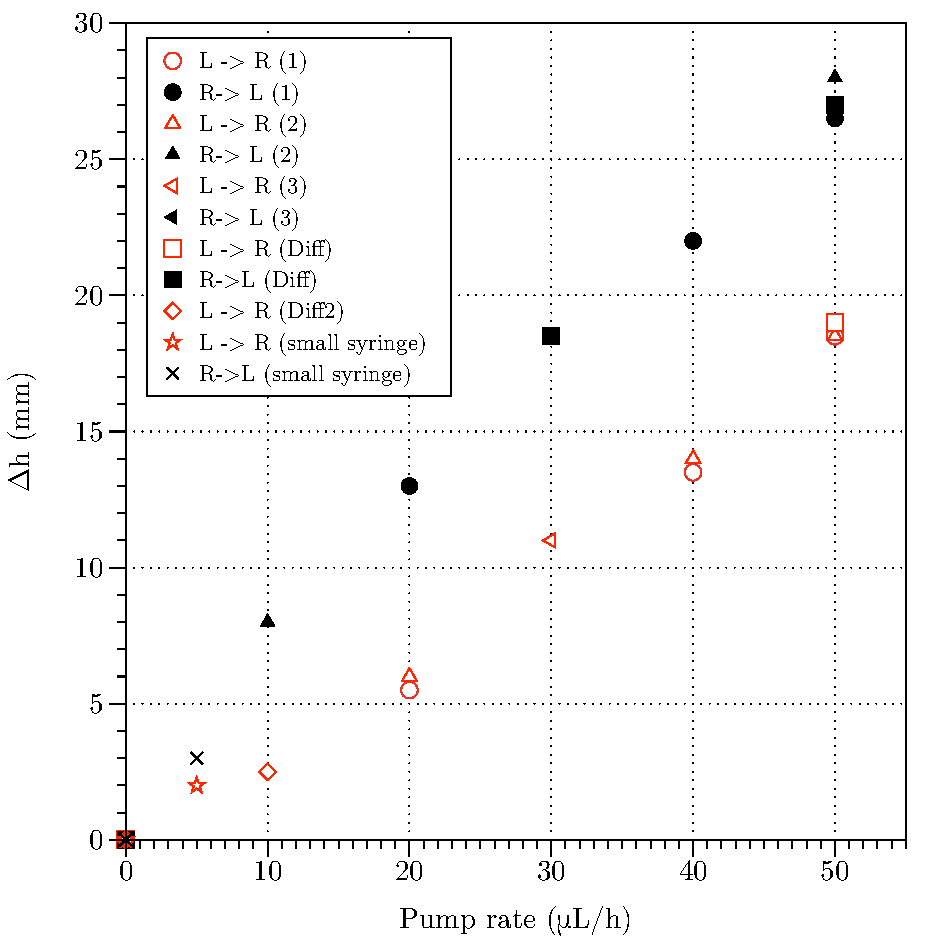
\includegraphics[width=0.8\textwidth]{Figures/Diode/first_diode/difference}
\end{center}
\caption[Difference in column heights as a function of flow rate for both directions (first diode behaviour)]{\label{fig:first_diode_main_graph}A plot of the difference in column height for flow in both directions as a function of the constant volumetric flow rate set at the syringe pump. For this cell, Left to Right (red) is the `easy' direction and Right to Left (black) is the `hard' direction. It is clearly visible that for all flow rates, a larger pressure is needed to achieve the same volumetric flow rate when flowing against the splay in the `hard' direction then is needed for flow in the `easy' direction.}
\end{figure}

After much repeated and sustained use of the diode cell from which the data points in Figure \ref{fig:first_diode_main_graph} were obtained, the parafilm spacer defining the cell channel failed, in conjunction with the development of a crack across the top face of the cell. This led to an unfixable leak in the cell which meant that no further data could be obtained, with particular reference to attempting to heat the system to the isotropic phase using the polystyrene housing and water heater as suggested earlier as being the key experiment in confirming that any diode like behaviour is due to the liquid crystal alignment.

A second diode cell was then created, adhering to the same fabrication conditions that are described for the cell above (rubbed at a rubbing parameter of 4.2 to produce approximately 45$^{\circ}$). The results from this cell are outlined in the next two sections.

\subsection{Second diode}
\label{sec:second_diode}
As stated above, a second diode cell was fabricated\footnote{Using the same rubbing conditions as the previous cell (rubbing parameter = 4.2).} and was set up the same way as the previous cell in the aluminium cell clamp shown in Figure \ref{fig:case} and polystyrene housing shown in Figure \ref{fig:heat_box_photos}. Again, preliminary experiments were conducted to estimate the column heights that would be measured when the syringe pump was set to different flow rates. Figure \ref{fig:second_diode_small_graphs} (a) to (d) show similar graphs to the previous cell in which the column heights are again plotted as a function of time and the volumetric flow rate set at the syringe pump. In particular, (c) and (d) show the columns reaching their equilibrium values when the smaller syringe is used, allowing for flow at the lowest volumetric flow rates.

\begin{figure}
\begin{center}
\subfigure[]{\includegraphics[width=0.49\textwidth]{Figures/Diode/second_diode/small_graphs1}}
\subfigure[]{\includegraphics[width=0.49\textwidth]{Figures/Diode/second_diode/small_graphs2}}
\subfigure[]{\includegraphics[width=0.49\textwidth]{Figures/Diode/second_diode/small_graphs3}}
\subfigure[]{\includegraphics[width=0.49\textwidth]{Figures/Diode/second_diode/small_graphs4}}
\end{center}
\caption[Calibration graphs for the second diode cell]{\label{fig:second_diode_small_graphs} (a) to (d) depict typical (there are many) calibration graphs whereby the range of column heights and flow rates are tested over several experiments. Again, column heights are plotted as a function of time and volumetric flow rate prescribed. These experiments allow the testing of different experimental set ups (as described earlier), and in (c) and (d) the use of the smaller diameter syringe in order to flow at lower volumetric flow rates.}
\end{figure}

With this cell, equilibrium column heights were measured by first filling the cell and manometer tubing at a high flow rate, and then gradually reducing the flow rate and allowing the column heights to come to their equilibrium values. Figure \ref{fig:second_diode_right_to_left} shows the experimental data for the complete set of volumetric flow rates in (a) the `easy' direction and (b) the `hard' direction, whereby the cell has been filled at a high flow rate and then sequentially dropped back in flow rate, tracking at the same time the height of the liquid crystal in both the left and right hand columns. This experiment is done in one flow direction at a time (i.e. the cell is filled and flown at all flow rates in the left to right direction. The flow is then stopped, the valve is moved to the second position, the columns are allowed to return to their equilibrium positions (where $\Delta h=0$ mm) and the flow is then started again in the opposite direction). Here it is shown that the cell was initially filled at a flow rate of 60 $\mu$L/h and sequentially dropped by 10 $\mu$L/h allowing for the column heights to become stable with time for both flow directions. This procedure resulted in manually reading the column heights every 30 minutes for a total of approximately 900 minutes. Again, this experiment was conducted in the polystyrene housing described earlier, but at this stage, was only run at room temperature (the water heater was not turned on). The effect of heating the system will be discussed in the next section. 

\begin{figure}
\begin{center}
\subfigure[]{\includegraphics[width=0.6\textwidth]{Figures/Diode/second_diode/left_to_right}}
\subfigure[]{\includegraphics[width=0.6\textwidth]{Figures/Diode/second_diode/right_to_left}}
\end{center}
\caption[Column heights as a function of time and flow rate (second diode)]{\label{fig:second_diode_right_to_left} (a) and (b) depict the column heights of the main experiment, whereby the flow is originally set at a high rate to fill the manometer tubes and then sequentially reduced, allowing the columns to reach their equilibrium values. (a) Flow from left to right (the `easy' direction) and (b)  flow from right to left (the `hard' direction).}
\end{figure}

Figure \ref{fig:second_diode_diff} shows a plot of the differences in the column heights as a function of the volumetric flow rate set at the syringe pump and the flow direction (taken from Figure \ref{fig:second_diode_right_to_left}). Here, flow in the `easy' direction (left to right) is plotted in red, and flow in the `hard' direction (right to left) is plotted in black. The different data sets shown in Figure \ref{fig:second_diode_diff} correspond to repeated attempts at the experiment and some `spot checks' whereby a particular flow rate and flow direction were tested again to determine if the value of $\Delta h$ initially measured was repeatable.

\begin{figure}
\begin{center}
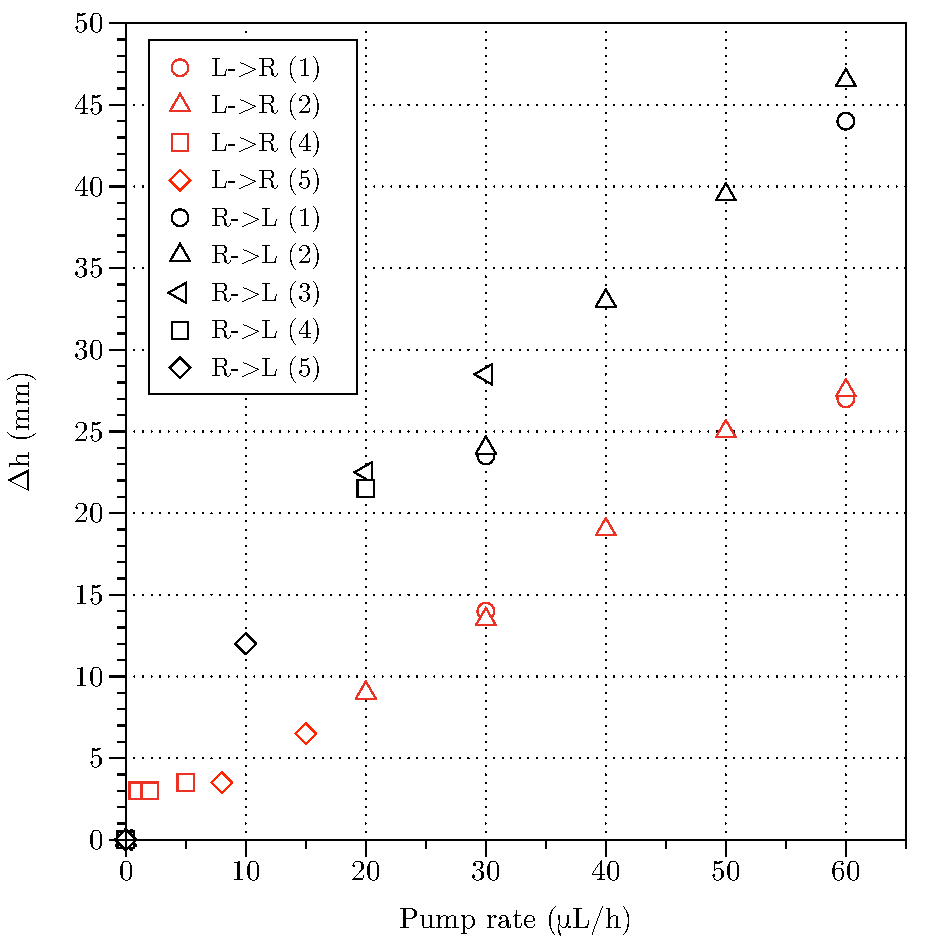
\includegraphics[width=0.7\textwidth]{Figures/Diode/second_diode/diff}
\end{center}
\caption[Difference in column heights as a function of flow rate for both directions (second diode behaviour)]{\label{fig:second_diode_diff} This graph is the equivalent of Figure \ref{fig:first_diode_main_graph} for the new diode cell. Here again, it is shown that for all pump rates, the column height difference, and hence the pressure gradient across the cell required, is lower for flow in the `easy' direction (left to right, red) then it is for flow in the `hard' direction (right to left, black). It is also seen that absolute values are comparable to the previous cell (shown in Figure \ref{fig:first_diode_main_graph}).}
\end{figure}

As can be seen, valve-like behaviour has been again recorded with a much larger column height difference measured at all volumetric flow rates for flow in the `hard' direction (black data sets). It is seen that Figure \ref{fig:second_diode_diff} closely resembles the results previously obtained for the previous diode cell in Figure \ref{fig:first_diode_main_graph}, demonstrating reproducibility of the experimental results under a slightly different method of data acquisition (filling the manometer tubes at the beginning under a high flow rate, before gradually reducing the flow rate). Likewise, the non-linear response of the pressure gradient as a function of flow rate has again been measured. Using the smaller syringe has also allowed for some data acquisition at the lowest flow rates, although due to experimental complications, these were only obtained for flow in the `easy' direction. 

As was set out earlier, a key test in determining whether or not any diode like behaviour measured is caused by the large splay and dynamic reorientation of the liquid crystal under flow in the `hard' direction, is to heat the cell to the isotropic phase and check flow in both directions. In the isotropic phase, it is expected that there should be no difference experienced by the liquid crystal between the flow directions, and an asymmetry in the pressure head required should not be present\footnote{This can not be guaranteed, as `pinning' of the director at the surfaces may affect the flow}. Up to this point, all experiments in this Chapter have been conducted at room temperature. The next section deals with using the polystyrene housing and water heater to raise the temperature of the enclosure to above the nematic - isotropic phase barrier whilst simultaneously attempting to measure the liquid crystal column heights for varying flow rates.

\subsection{Isotropic phase}
\label{sec:isotropic}

To begin with, all experimental data presented in this section is taken from the same cell that is used in the previous Section (\ref{sec:second_diode}) (the second cell to exhibit diode like behaviour).

Due to unforeseen time constraints and equipment problems, there was a large gap of several weeks between the data acquisition in Section \ref{sec:second_diode} and the commencement of the experiments described in the section involving heating the system to the isotropic phase. As such, when returning to the experimental set up and apparatus, a quick calibration experiment was conducted to ensure that the cell was still responding in the same way as previously measured. Figure \ref{fig:isotropic_check} shows the results of this check. A spot test was made at a flow rate of 60 $\mu$L/h, whereby the cell was originally flown in the `easy' (left to right) direction before being switched to flow in the `hard' (right to left) direction. Here it is shown that after approximately 180 minutes in the `easy' direction the cell has reached an equilibrium value of $\Delta h= 29$ mm (compared to $\Delta h= 27$ mm from Figure \ref{fig:second_diode_diff}), and after approximately another 200 minutes in the `hard' direction, the cell has reached an equilibrium value of $\Delta h= 42$ mm (compared to $\Delta h= 45$ mm from Figure \ref{fig:second_diode_diff}). So it is established that the cell still responds in a similar manner to earlier\footnote{A comparison of the individual left and right column heights at 60 $\mu$L/h shown in both Figures \ref{fig:isotropic_check} and \ref{fig:second_diode_right_to_left} also yields the same results.}. With this result confirmed, experiments involving the heating of the cell could now be undertaken.

\begin{figure}
\begin{center}
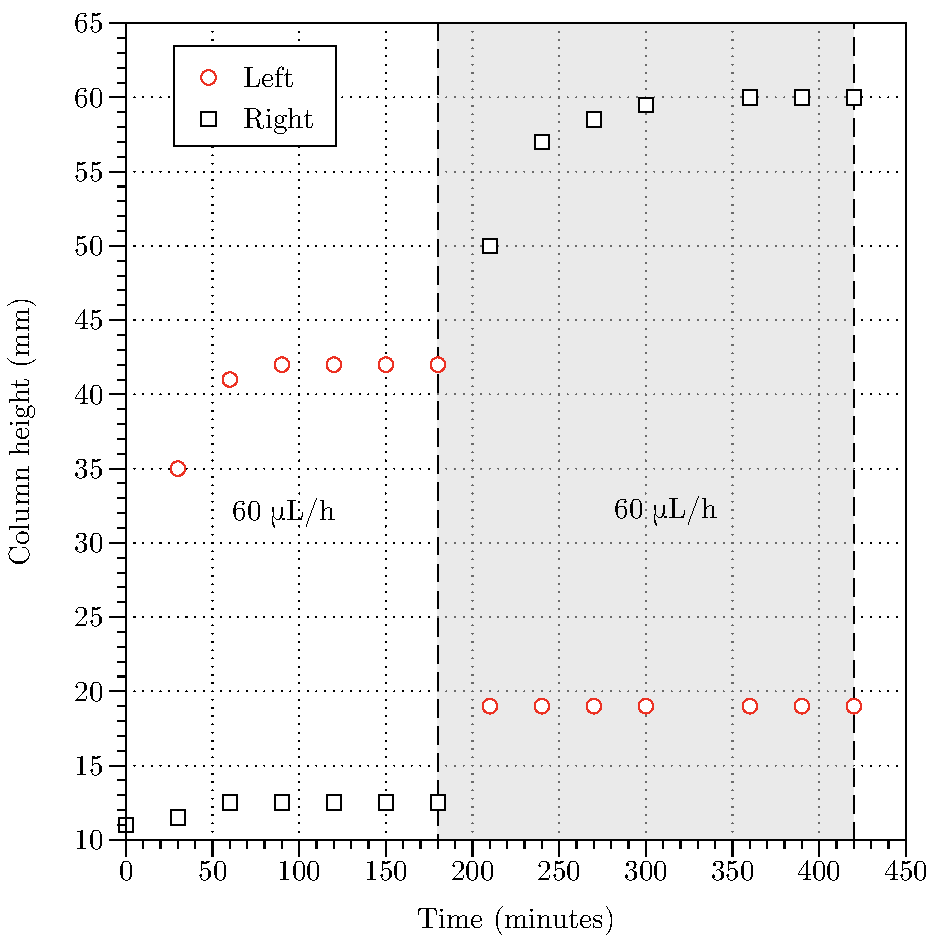
\includegraphics[width=0.7\textwidth]{Figures/Diode/second_diode/isotropic/check_same_as_before}
\end{center}
\caption[Second diode repeat experiment]{\label{fig:isotropic_check} Due to the amount of time between the data shown in Figure \ref{fig:second_diode_diff} and the isotropic phase experiment, a quick calibration experiment was carried out. This plot shows that the cell is still behaving in the same fashion as before, with both the left and right column heights reaching the same values as previously (Figure \ref{fig:second_diode_diff}), with values of $\Delta h$ reaching $\approx29$ mm for left to right at 60 $\mu$L/h and $\approx40$ mm for right to left at 60 $\mu$L/h.}
\end{figure}

\subsection{Heating the cell}
Due to the delicate nature of the liquid crystal flow cells described in this thesis, their tendency to fracture, and the length of time this experiment had been running, it is fair to say that there was some apprehension when beginning the heating of the the housing to $T_{N-I}$ (approximately 35 $^{\circ}\text{C}$ for 5CB \cite{Skarp1979}). The reason for this was a concern over the expansion of the cell due to the increased temperature, leading to increased stress and as the cell is maintained in a clamp, this could cause it to crack or weaken. Also, the raised temperature environment changes the mechanical properties of all components of the experiment and could have any number of unknown effects on the equipment. Another reason for conducting this preliminary experiment was in order to establish how the polystyrene housing responds to the water heater, with particular respect to how fast the box heats up, what temperature the water needs to achieve for the required temperature in the box and how stably can the temperature in the box be maintained?

Thus, the first experiment conducted was to heat the cell only to 30 $^{\circ}\text{C}$ as a trial. The results of this experiment are plotted in Figure \ref{fig:30}. Here, Figure \ref{fig:30} (a) depicts the column heights as before, whilst Figure \ref{fig:30} (b) gives the temperature of the water in the heater (downwards blue triangle) and the air temperature of the box measured next to the cell (upwards black triangle). The $x$ axis (time) on both (a) and (b) are identical, meaning that a direct comparison between the temperature of the enclosure and the column height can be easily made by following a straight line vertically up or down to the other graph.

To begin with, as shown in Figure \ref{fig:30} (a), the syringe pump is set at a flow rate of 60 $\mu$L/h, pumping from left to right through the cell. After 100 minutes, the heights have reached their equilibrium values of 40 mm and 12 mm, creating a column height difference of $\Delta h=28\text{ mm}$ (as expected from Figure \ref{fig:isotropic_check}). At this point, the water in the heater is turned on to pump around the housing and is set to be at a temperature of approximately 28 $^{\circ}$C (see Figure \ref{fig:30} (b)). Here it is seen that the water temperature quickly reaches the desired value of 30 $^{\circ}\text{C}$ (blue triangles), whereas the air temperature in the box slowly increases over approximately 30 minutes (black triangles). After this point, the temperature of the water from the heater had to be significantly reduced to approximately 25 $^{\circ}\text{C}$ in order to maintain the air temperature in the box at approximately 30 $^{\circ}\text{C}$. The reason for this, was the unforeseen heating caused by the syringe drive. In the confined and enclosed space, the heat given off by the motor in the syringe drive is enough to significantly heat the air in the enclosure. It was found that maintaining the required air temperature within the enclosure involved a delicate balancing raising or lowering the water temperature accordingly.

\begin{figure}
\begin{center}
\subfigure[]{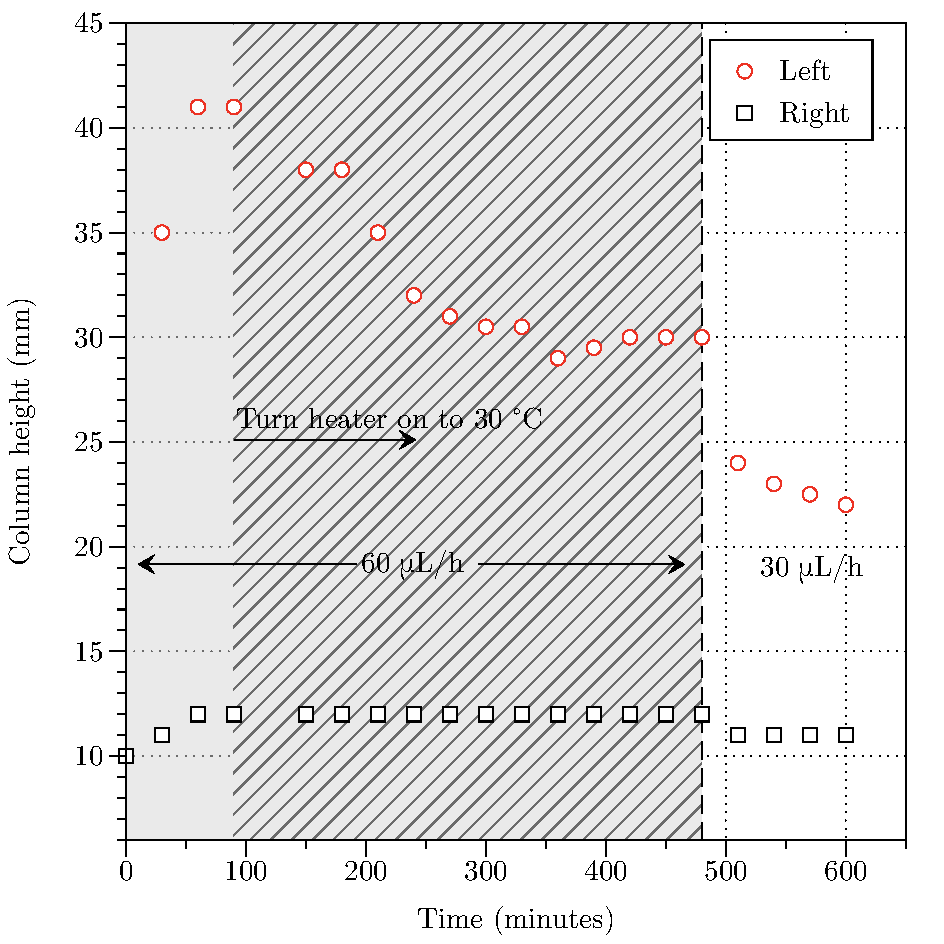
\includegraphics[width=0.6\textwidth]{Figures/Diode/second_diode/isotropic/30}}
\subfigure[]{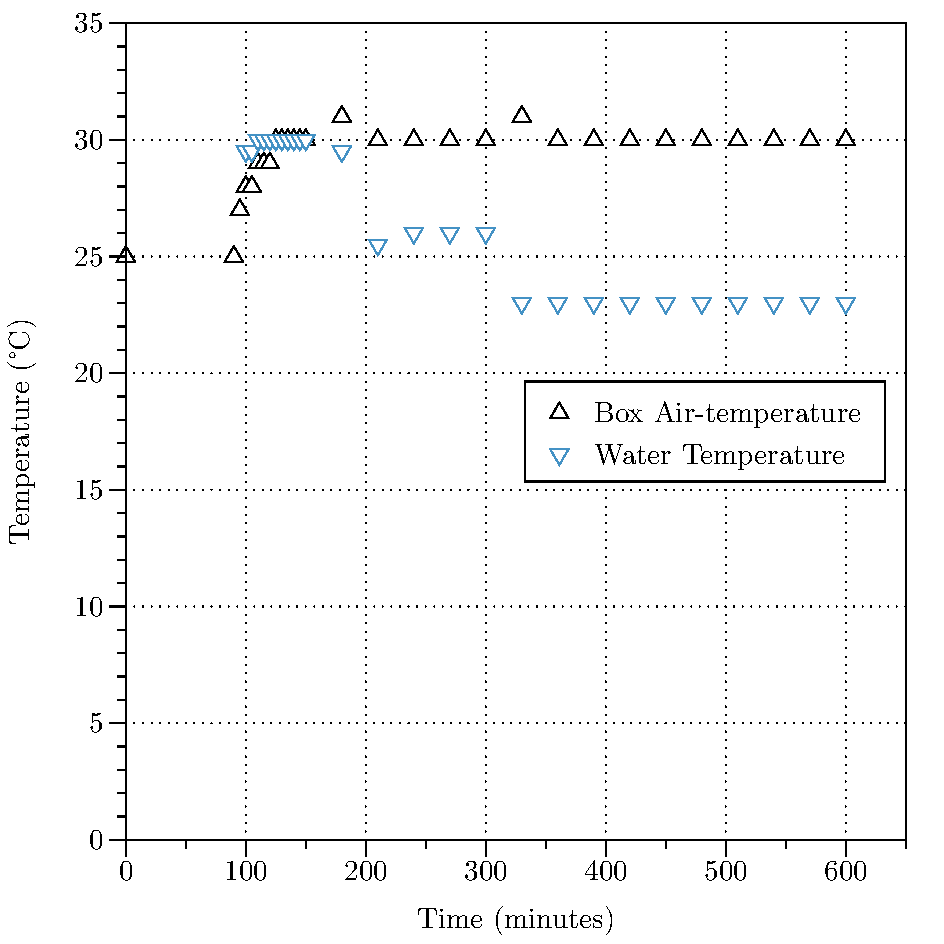
\includegraphics[width=0.6\textwidth]{Figures/Diode/second_diode/isotropic/30_temp}}
\end{center}
\caption[Heat system to 30 $^{\circ}\text{C}$]{\label{fig:30}(a) depicts the relative column heights as a function of time and volumetric flow rate when the temperature of the enclosure has been raised to approximately 30 $^{\circ}\text{C}$. (b) shows the temperature of the water from the heater that is circulated around the bottom plate of the enclosure (blue triangles) and the measured air temperature in the box from the thermocouple thermometer (black triangles) as a function of time. Note that the $x$ axis on both (a) and (b) are identical so an easy comparison can be made between a specific time and temperature or column height by drawing a vertical line between the two graphs.}
\end{figure}

As is seen in Figure \ref{fig:30} (a), as the temperature of the air in the box begins to increase, the height of liquid crystal in the column begins to decrease\footnote{Note that there has been no change in the flow rate set at the syringe drive}. That is to say that, the pressure head needed for the same volumetric flow rate has significantly decreased due to the reduced viscosity of the liquid crystal at the higher temperature, as will be discussed later. It can also be seen that this change in the column height took nearly 450 minutes to stabilise at a new height difference of  $\Delta h=17\text{ mm}$. The `noisy' nature of the left column height measurement between $t=100\text{ m}$ and $t=480\text{ m}$ is probably due to the difficulty in physically making an accurate reading of the height of the liquid crystal in the column. This is due to the fact that for this (and any future) temperature controlled experiment, the polystyrene enclosure is fully sealed as depicted in Figure \ref{fig:heat_box_photos} (b). To undertake a measurement, a flap near the top of the box is opened, and using a torch, the column height is read against the ruler at the back of the manometer tubing. Performing this measurement can be difficult, particularly with the time constraint for not allowing the enclosure to significantly cool whilst a measurement is being taken. It will also be seen that this measurement is made slightly more difficult in the isotropic phase where it is very difficult to see the liquid crystal in the manometer tubing.

\subsection{Isotropic experiment}
\label{sec:iso_experiment}
After becoming familiar with the experimental method of heating the enclosure and maintaining the temperature whilst taking readings from the manometer tubing, the cell could now be heated to the isotropic phase and the experiment of Section \ref{sec:second_diode} repeated.

Figure \ref{fig:isotropic_left_to_right} (a) shows a plot, similar to that of Figure \ref{fig:30} (a) (where the enclosure was heated to 30 $^{\circ}\text{C}$) but this time the enclosure has been heated to 35 $^{\circ}\text{C}$ (above $T_{N-I}$ for 5CB) as is shown in Figure \ref{fig:isotropic_left_to_right} (b) for flow in the 'easy' (left to right) direction. Again, the experiment begins by setting the syringe pump to 60 $\mu$L/h and allowing the liquid crystal in the manometer columns to come to their equilibrium values. At this point the water heater is switched on and the air temperature in the box begins to increase. This temperature increase results in a drop of the column heights to a new equilibrium value (approximately $\Delta h=18\text{ mm}$ in Figure \ref{fig:isotropic_left_to_right} (a) at $t=560\text{ m}$). It can be seen from \ref{fig:isotropic_left_to_right} (b) that the system enters the isotropic phase at approximately $t=250\text{ m}$ (which is also visually confirmed by the liquid crystal becoming clear).

Now that the system is completely in the isotropic phase (the liquid crystal in all tubing, the cell and syringe, is visually confirmed to have become clear) the similar experimental method of reducing the flow rate at the syringe pump and tracking the column heights as a function of time is employed. Here, again, due to the experiment taking almost 17 hours to run (with manual column height reading every 30 minutes) and a finite amount of liquid crystal in the syringe, flow rates of 60 $\mu$L/h, 40 $\mu$L/h and 20 $\mu$L/h could be measured. Figure \ref{fig:isotropic_left_to_right} (b) also confirms that the temperature within the enclosure (black triangles) stayed above $T_{N-I}$ for the duration of the experiment.

\begin{figure}
\begin{center}
\subfigure[]{\includegraphics[width=0.6\textwidth]{Figures/Diode/second_diode/isotropic/left_to_right}}
\subfigure[]{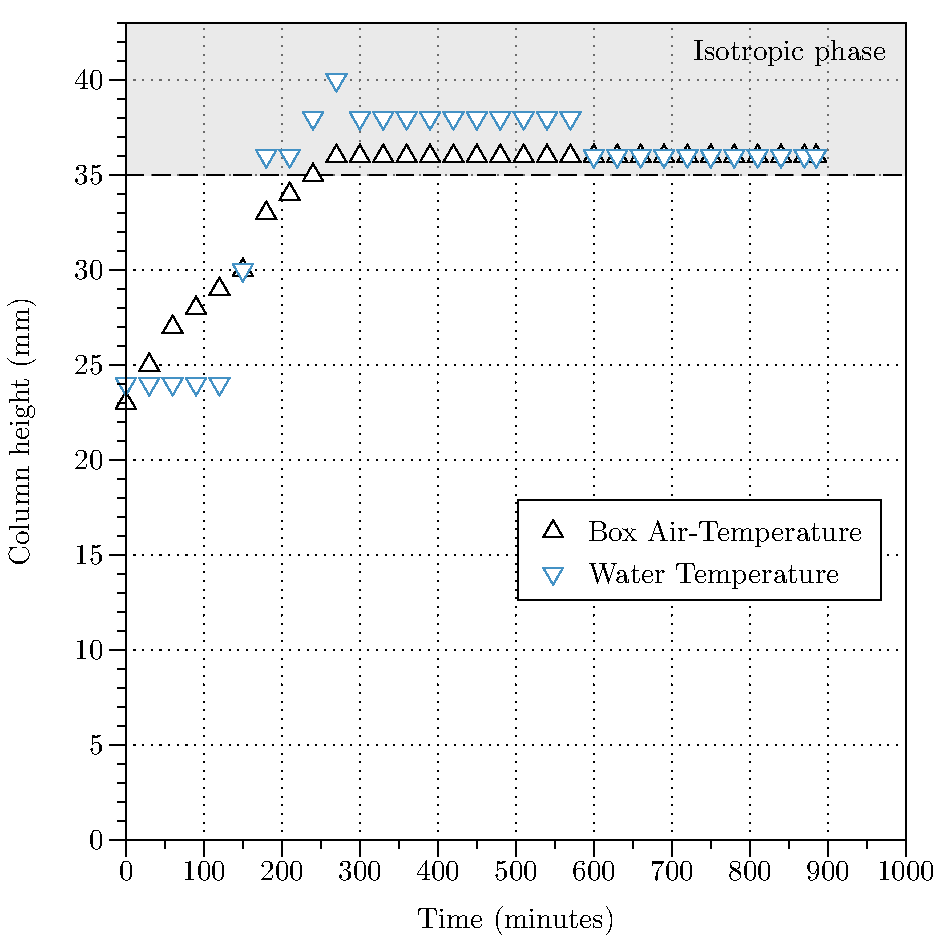
\includegraphics[width=0.6\textwidth]{Figures/Diode/second_diode/isotropic/left_to_right_temp}}
\end{center}
\caption[Column heights in the isotropic phase (left to right)]{\label{fig:isotropic_left_to_right}(a)depicts the relative column heights as a function of time and volumetric flow rate when the temperature of the enclosure has been raised to over 35 $^{\circ}\text{C}$ ($T_{N-I}$ for 5CB). (b) shows the temperature of the water from the heater that is circulated around the bottom plate of the enclosure (blue triangles) and the measured air temperature in the box from the thermocouple thermometer (black triangles) as a function of time. Temperatures above $T_{N-I}$ are shaded in grey. Note that the $x$ axis on both (a) and (b) are identical so an easy comparison can be made between a specific time and temperature or column height by drawing a vertical line between the two graphs.}
\end{figure}

\begin{figure}
\begin{center}
\subfigure[]{\includegraphics[width=0.6\textwidth]{Figures/Diode/second_diode/isotropic/right_to_left}}
\subfigure[]{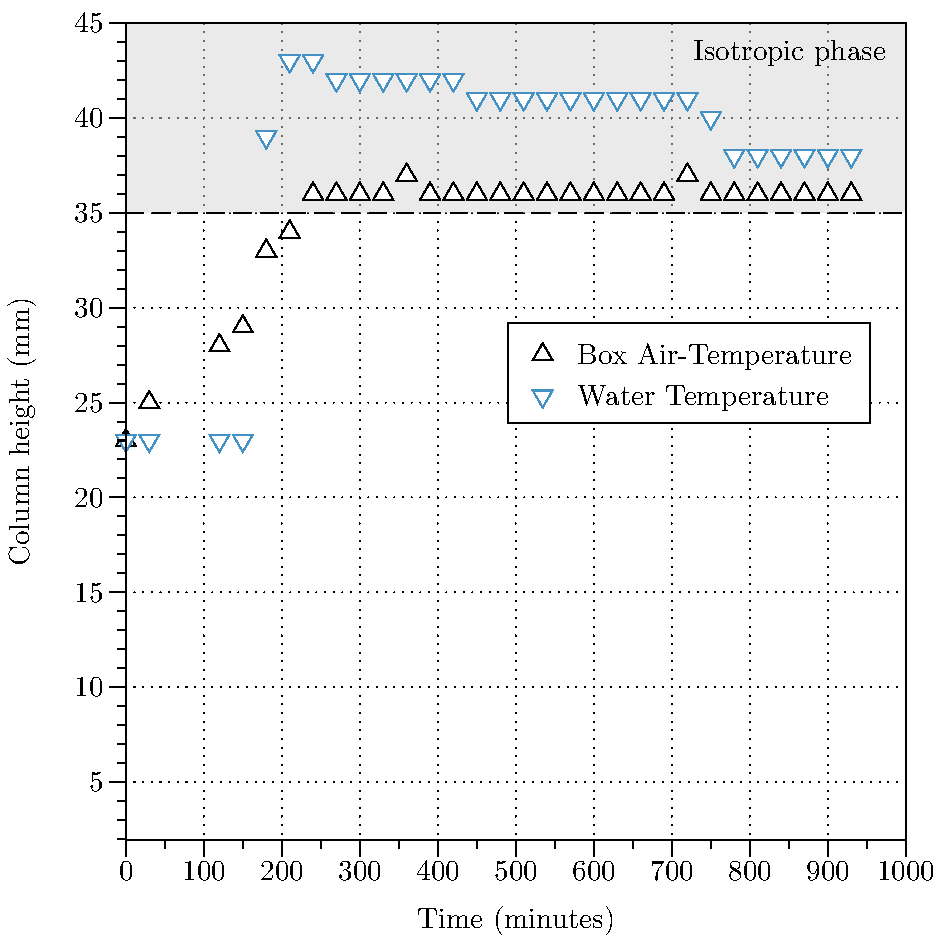
\includegraphics[width=0.6\textwidth]{Figures/Diode/second_diode/isotropic/right_to_left_temp}}
\end{center}
\caption[Column heights in the isotropic phase (right to left)]{\label{fig:isotropic_right_to_left}(a) depicts the relative column heights as a function of time and volumetric flow rate when the temperature of the enclosure has been raised to over 35 $^{\circ}\text{C}$ ($T_{N-I}$ for 5CB). (b) shows the temperature of the water from the heater that is circulated around the bottom plate of the enclosure (blue triangles) and the measured air temperature in the box from the thermocouple thermometer (black triangles) as a function of time. Temperatures above $T_{N-I}$ are shaded in grey. Note that the $x$ axis on both (a) and (b) are identical so an easy comparison can be made between a specific time and temperature or column height by drawing a vertical line between the two graphs.}
\end{figure}

Figure \ref{fig:isotropic_right_to_left} (a) shows the same plot for flow in the `hard' (right to left) direction, again where the flow has initially been started at 60 $\mu$L/h in the liquid crystalline phase. After approximately 220 minutes the system enters the isotropic phase, as shown in Figure \ref{fig:isotropic_right_to_left} (b), upon which the column heights for flow at 60 $\mu$L/h begin to reduce. Again, flow rates were then sequentially reduced through 40 $\mu$L/h and 20 $\mu$L/h until all of the liquid crystal in the syringe had been used up. The noise associated with the curves in Figure \ref{fig:isotropic_right_to_left} (a) is again accredited to the physical difficulty in making an accurate reading. Also, some small fluctuations in the air temperature of the box are seen in Figure \ref{fig:isotropic_right_to_left} (b) which are again due to the manual balancing act between the water temperature and the heat given off by the syringe drive, mixed in with the slight cooling of the system every time the lid is opened to read a measurement from the manometer tubes.

\begin{figure}
\begin{center}
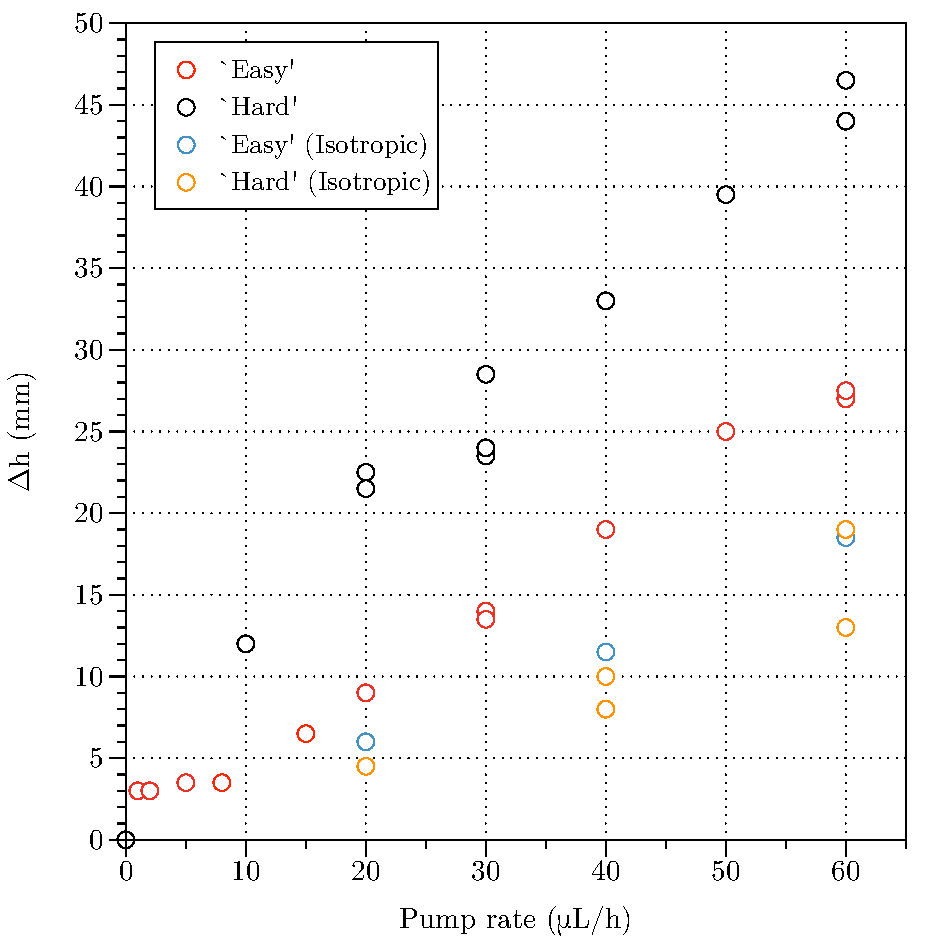
\includegraphics[width=0.7\textwidth]{Figures/Diode/second_diode/isotropic/iso_diff}
\end{center}
\caption[Summary of column height differences in nematic and isotropic phases]{\label{fig:iso_diode_diff} A comparison between the column height differences measured for flow in both the `easy' and `hard' directions in both the liquid crystalline and isotropic phases. A clear reduction in the column height difference is seen to occur at all flow rates in the isotropic phase, with a much smaller asymmetry in the column height difference measured for the two flow directions.}
\end{figure}

Figure \ref{fig:iso_diode_diff} collates all of the data taken from the second diode cell and plots the column height difference as a function of the volumetric flow rate set at the syringe and the direction of flow through the cell. Flow in the `easy' and `hard' directions whilst in the liquid crystalline phase  are shown by the red and black data sets respectively (the same data sets plotted in Figure \ref{fig:second_diode_diff}). Flow in the `easy' and `hard' directions whilst in the isotropic phase are shown by the blue and orange data sets respectively (with the values of $\Delta h$ taken from Figures \ref{fig:isotropic_left_to_right} and \ref{fig:isotropic_right_to_left}). It is shown that in the isotropic phase, the column height difference is much lower for flow in the liquid crystalline phase for flow in both the `easy' and `hard' directions. The difference between the column heights measured for flow in both directions is also much smaller, but still seems to be present (the two orange data sets correspond to the original described above, and a repeat of the isotropic experiment flown in the `hard' direction). 

\section{Director profiles}
The premise of using the dynamic reorientation of the director as a means of creating a flow cell that has a preferential flow direction is here envisioned by creating a large pretilt angle on both surfaces so that the director profile forms a splay in $z$. Such a director profile would be described as having a large pretilt at the cell walls, going through planar at the cell mid-plane (if the value of the pretilt angle were to be identical on both surfaces). However, another stable director profile that could be formed is that of the bend state, whereby, the director has a large pretilt at the aligning surfaces, but remains vertically aligned at the cell mid-plane.

As was touched upon briefly in Chapter \ref{cha:pretilt}, work by Yeung \textit{et al} \cite{Yeung2006,Yu2004,Yeung2005} on the production of the no-bias-bend (NBB) $\pi$-cell and the \textit{bistable} bend-splay device has shown how the elastic deformation of energy of both the splayed and bend state can be very similar, if not identical, for a pretilt angle of $45^{\circ}$ \cite{Yeung2005}. Since in this chapter we are fabricating cells with similarly large pretilt angles, it is relevant to determine wether or not the diode cells have formed a static splay or bend geometry before the flow begins.

\subsection{Fully Leaky Guided Modes}
To begin with, it was desirable to accurately determine the director profile as a function of the cell depth in order to help gain a high definition insight into the response and behaviour of the cell once dynamic experiments were started. In order to do this, attempts were made to characterise the director profile by use of the Fully Leaky Guided Mode (FLGM) technique, which has been used extensively before at the University of Exeter \cite{Cornford2009,Yang2007,Jewell2005a,Jewell2006,Jewell2007}. Briefly explained, guided modes through the cell are measured in reflection and transmission over a range of incident angles as a function of the incident and detected polarisation. This results in an extremely large data set consisting of $R_{ss},R_{sp},R_{ps},R_{pp},T_{ss},T_{sp},T_{ps},T_{pp}$ where the first subscript denotes the incident polarisation and the second subscript denotes the detected polarisation. For example $R_{sp}$ corresponds to the reflected signal that was detected as $p$ polarised when the incident beam was initially $s$ polarised, and in this case, polarisation conversion must have occurred for there to be any signal detected. From such a large data set, a computational fitting routine can be employed to (using the known parameters such as the elastic constants and refractive indices) fit the director profile through the cell. With such a large data set, any degeneracies in detected signals should be avoided. 

Due to the extreme sensitivity of the FLGM technique to subtle variations in cell thickness \cite{Taphouse2007} (which are certainly present in a flow cell constructed from parafilm walls) which are easily sampled by a slightly rastering beam spot (particularly at high incidence angle) and non uniform director alignment (certainly present, as shown in Chapter \ref{cha:pretilt} for `over-baked' Nissan SE-1211 and later on in this chapter) and the time involved with highly accurate data acquisition and fitting routines, it was decided not to use this approach but instead examine it using conoscopy. However, including a note on the FLGM technique in this thesis is warranted due to the amount of time spent trying to characterise potential `diode cells'.

Conoscopic figures from the experimental cell were compared to simulated figures for both the bend and splay state in order to determine which was present in the diode cell used. The details of this investigation follow.

\subsection{Bend state (vertical at cell mid-plane)}
Figure \ref{fig:vertical_middle} (a) - (c) shows simulated conoscopic interference figures for the director profiles schematically depicted beneath in (d) - (f). For a cell that is fully vertically aligned (a), the conoscopic figure is the classic Maltese cross as is expected as described earlier in this thesis. As the pretilt angle at the surface is moved towards planar, with the director constrained to be vertical at the mid-plane, the bend state is observed (b), where a complex and distorted conoscopic figure is simulated with distorted black lobes appearing to spread vertically across the field of view. This figure is shown to distort even more dramatically as the director is forced to be planar at the cell walls but remain vertically aligned at the cell mid-plane (a highly unrealistic director profile) (c). Here it is shown that for maintained vertical alignment at the cell mid-plane, very distinct conoscopic figures are expected.
\begin{figure}
\begin{center}
\subfigure[]{\includegraphics[width=0.2\textwidth]{Figures/Diode/second_diode/conoscopy/vertical_middle/1}}
\subfigure[]{\includegraphics[width=0.2\textwidth]{Figures/Diode/second_diode/conoscopy/vertical_middle/4}}
\subfigure[]{\includegraphics[width=0.2\textwidth]{Figures/Diode/second_diode/conoscopy/vertical_middle/7}}\\
\subfigure[]{\includegraphics[width=0.14\textwidth]{Figures/Diode/second_diode/conoscopy/vertical_middle/a}}\hspace{9mm}
\subfigure[]{\includegraphics[width=0.14\textwidth]{Figures/Diode/second_diode/conoscopy/vertical_middle/b}}\hspace{9mm}
\subfigure[]{\includegraphics[width=0.14\textwidth]{Figures/Diode/second_diode/conoscopy/vertical_middle/c}}
\end{center}
\caption[Simulated conoscopic figures - director vertical at mid-plane]{\label{fig:vertical_middle}Figures (a) - (c) depict simulated conoscopic interference figures where by the director profile varies as schematically depicted in (d)-(f) directly below, respectively. Here, the pretilt angle varies from vertical to planar whilst being constrained to remain vertical at the cell mid-plane.}
\end{figure}

\subsection{Splay state (planar at cell mid-plane)}
Figure \ref{fig:planar_middle} (a) - (c) also shows simulated conoscopic interference figures for the director profiles schematically depicted beneath in (d) - (f). Again, the simulated figures go from vertical pretilt angles to planar pretilt angles but this time the cell is forced to remain planar at the cell mid-plane. For the cell that is aligned vertically at the cell walls and planar at the cell mid-plane (a) a broadly white and featureless figure is simulated, with a slight darkening in the middle and the left and right hand edges. As the pretilt angle is moved towards planar at the cell walls, the splayed director profile is observed (b) (the desirable director profile for this experiment) where a dark area is observed in the centre of the figure which appears to be two fringes from the top and bottom meeting in the middle. Finally, as the pretilt angle reaches full planar alignment, the expected conoscopic figure of a double set of hyperbolae is recovered.

\begin{figure}
\begin{center}
\subfigure[]{\includegraphics[width=0.2\textwidth]{Figures/Diode/second_diode/conoscopy/planar_middle/1}}
\subfigure[]{\includegraphics[width=0.2\textwidth]{Figures/Diode/second_diode/conoscopy/planar_middle/4}}
\subfigure[]{\includegraphics[width=0.2\textwidth]{Figures/Diode/second_diode/conoscopy/planar_middle/7}}\\
\subfigure[]{\includegraphics[width=0.14\textwidth]{Figures/Diode/second_diode/conoscopy/planar_middle/a}}\hspace{9mm}
\subfigure[]{\includegraphics[width=0.14\textwidth]{Figures/Diode/second_diode/conoscopy/planar_middle/b}}\hspace{9mm}
\subfigure[]{\includegraphics[width=0.14\textwidth]{Figures/Diode/second_diode/conoscopy/planar_middle/c}}
\end{center}
\caption[Simulated conoscopic figures - director planar at mid-plane]{\label{fig:planar_middle} Figures (a) - (c) depict simulated conoscopic interference figures where by the director profile varies as schematically depicted in (d)-(f) directly below, respectively. Here, the pretilt angle varies from vertical to planar whilst being constrained to remain planar at the cell mid-plane.}
\end{figure}

Importantly, it is clear that the conoscopic figures from the two alignment states should appear distinctly different, resulting in relatively simple classification of the director profile present in the diode cells used for flow experiments in this chapter.

\subsection{Data}
Figures \ref{fig:diode_director} (a) and (b) show CCD captures from the conoscope for the diode cell used in the diode flow experiments described in Section \ref{sec:second_diode}. Images (a) and (b) \textit{are taken from different areas of the flow channel}. Immediately it is clear that as the centre of these conoscopic figures is translated away from the centre of the field of view, the cell has a non-mirror symmetric director profile about the cell mid-plane, but crucially it is also seen that the figures are made of two sets of fringes that appear to be distorted (characteristic of the conoscopic figure for the splayed profile depicted in Figure \ref{fig:planar_middle} (e)). 

It is known from the experimental data in Chapter \ref{cha:pretilt} that the pretilt angle of the director should be on the order of $40^{\circ}$ to $50^{\circ}$ away from the surface, so by estimating an asymmetric pretilt angle of $50^{\circ}$ away from the surface on the bottom face and $40^{\circ}$ away from the surface on the top face (but still forming a splayed director profile), simulated figures such as those shown in Figures \ref{fig:diode_director} (c) and (d) are obtained. This seems to suggest (by no means rigorously) that the actual director profile in the diode cells that have been used are exhibiting a splay (where the director goes through planar alignment at some point close to the cell mid-plane), with a slightly different value of pretilt angle on each surface (although both are around $40^{\circ}$ to $50^{\circ}$). The similarity between Figures \ref{fig:diode_director} (a) and (c) (data and simulation) and Figures \ref{fig:diode_director} (b) and (d) (data and model) are clear, and also hint at the fact that the value of the pretilt angles obtained are not uniform across the length of the flow channel.

This exercise is not intended to give a highly detailed analysis of the director profile whereby the exact angle of the director as a function of cell depth can be determined accurately. It is simply intended to provide some idea of the actual director profile (with regards to splay and bend) that is actually exhibited in the cell in order to attempt some simulation of the director profiles under flow using Ericksen-Leslie theory as described and used in pervious chapters.

\begin{figure}
\begin{center}
\subfigure[]{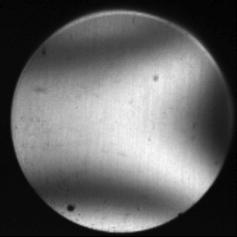
\includegraphics[width=0.2\textwidth]{Figures/Diode/second_diode/conoscopy/data_1}}
\subfigure[]{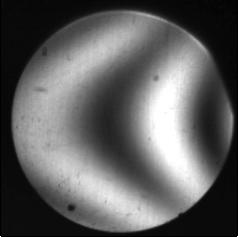
\includegraphics[width=0.2\textwidth]{Figures/Diode/second_diode/conoscopy/data_2}}\\
\subfigure[]{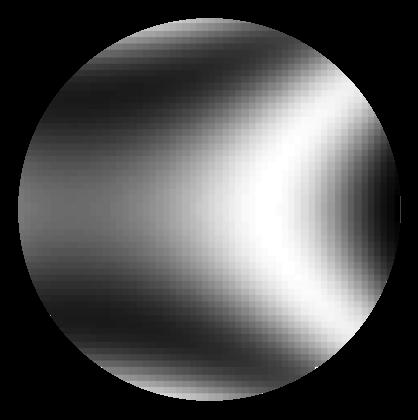
\includegraphics[width=0.2\textwidth]{Figures/Diode/second_diode/conoscopy/model_1}}
\subfigure[]{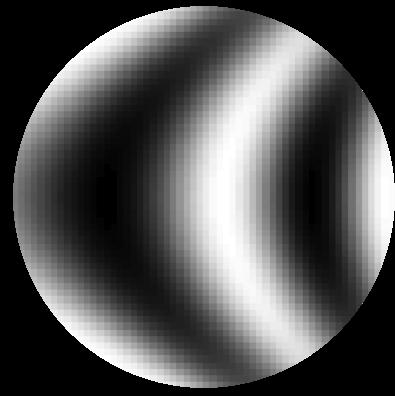
\includegraphics[width=0.2\textwidth]{Figures/Diode/second_diode/conoscopy/model_2}}
\end{center}
\caption[Comparison between experimental and simulated splayed conoscopic figures]{\label{fig:diode_director}Figures (a) and (b) show conoscopic interference figures for different areas of the second diode cell (used in Section \ref{sec:second_diode}). Figures (c) and (d) are simulated conoscopic figures for pretilt angles of approximately 45$^{\circ}$ (splayed) on each surface. In order to translate the centre of the interference figure, the pretilt angle has to be slightly asymmetric about the cell mid-plane.}
\end{figure}

The final section of this chapter will now go on to make a comparison between the data obtained and the predictions from the one dimensional model, allowing simulated director profiles to be analysed.

\section{Simulation}
\subsection{Planar}
Figure \ref{fig:diode_planar} shows the simulated director profiles for a cell that is initially aligned planar and parallel to the flow direction. (a) the director tilt profiles as a function of volumetric flow rate and flow direction, (b) the velocity profiles as a function of volumetric flow rate and flow direction and (c) the pressure gradient as a function of the volumetric flow rate (all figures show curves at regular pressure gradient intervals ranging from blue (no flow) to yellow (maximum flow), going through orange). For the following graphs of volumetric flow rate vs. pressure gradient, the volumetric flow rate has been plotted as negative values for flow against the splay (`hard') and positive values for flow with the splay (`easy'). This enables an easy comparison between the difference in the pressure gradient required to achieve the same volumetric flow rate (on either side of the $y$ axis).

It is seen in Figure \ref{fig:diode_planar} (a) that as expected, for flow in both directions, the director rotates to achieve the steady state Leslie angle of opposite sign in the bottom and top halves of the cell. This is shown by the saturation of the tilt distortion at values of approximately $79^{\circ}$ and $101^{\circ}$ (both approximately $11^{\circ}$ away from planar) as has been previously described in Chapter \ref{cha:45}. Figure \ref{fig:diode_planar} (b) also shows the associated velocity profiles for flow in both directions. Again, as expected, there is no difference in the magnitude and shape of the velocity distribution for flow in either direction. Finally, Figure \ref{fig:diode_planar} (c) depicts the calculated volumetric flow rate for the pressure gradient prescribed in the simulation. Here it is clear that for flow in both directions, the relation between the pressure gradient and the volumetric flow rate is linear and identical. Of course, this is exactly as expected. For a flow channel where the director is aligned planar and parallel to the flow direction, there is no asymmetry to cause a difference in the response of the cell to a change in the flow direction.

\begin{figure}
\begin{center}
\subfigure[Tilt profile]{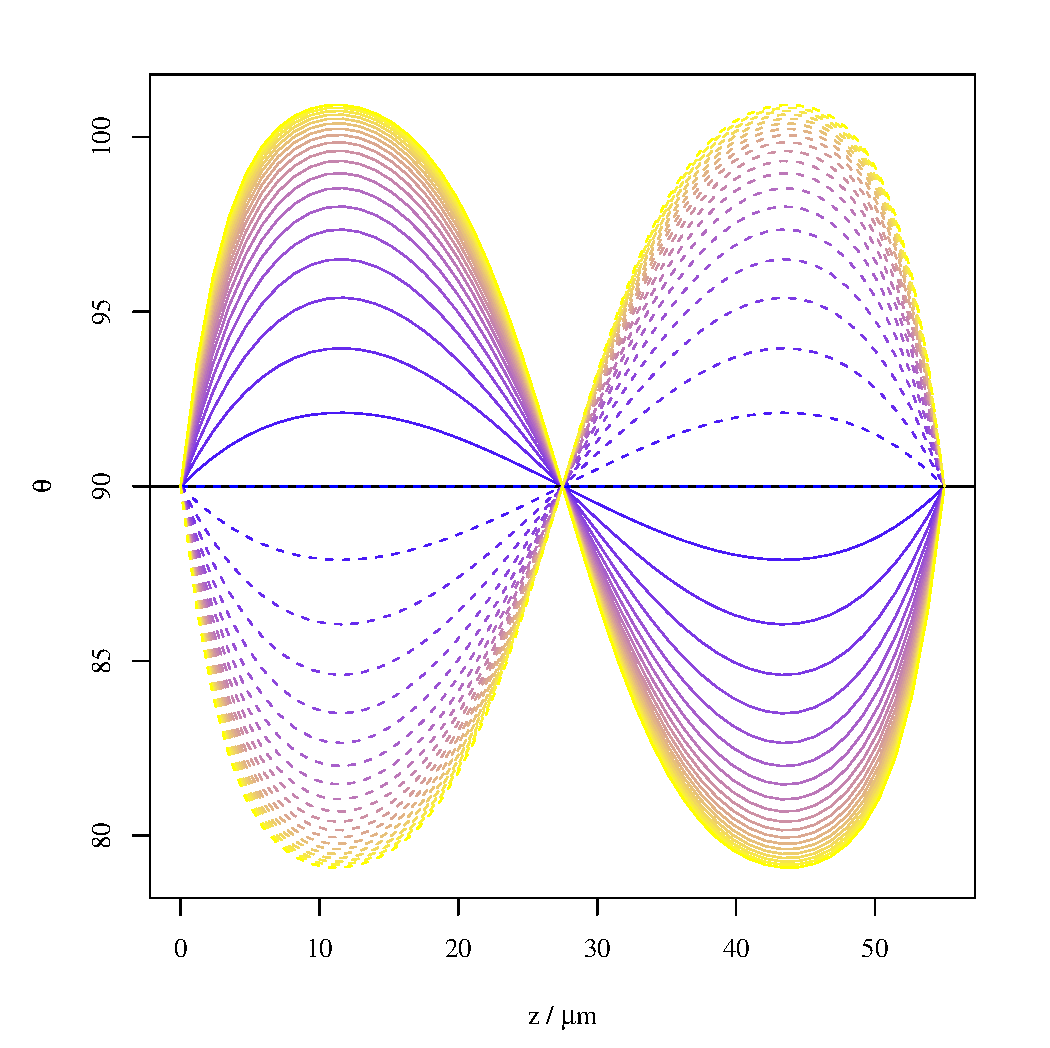
\includegraphics[width=0.49\textwidth]{Figures/diode/model/planar_tilt}}
\subfigure[Velocity profile]{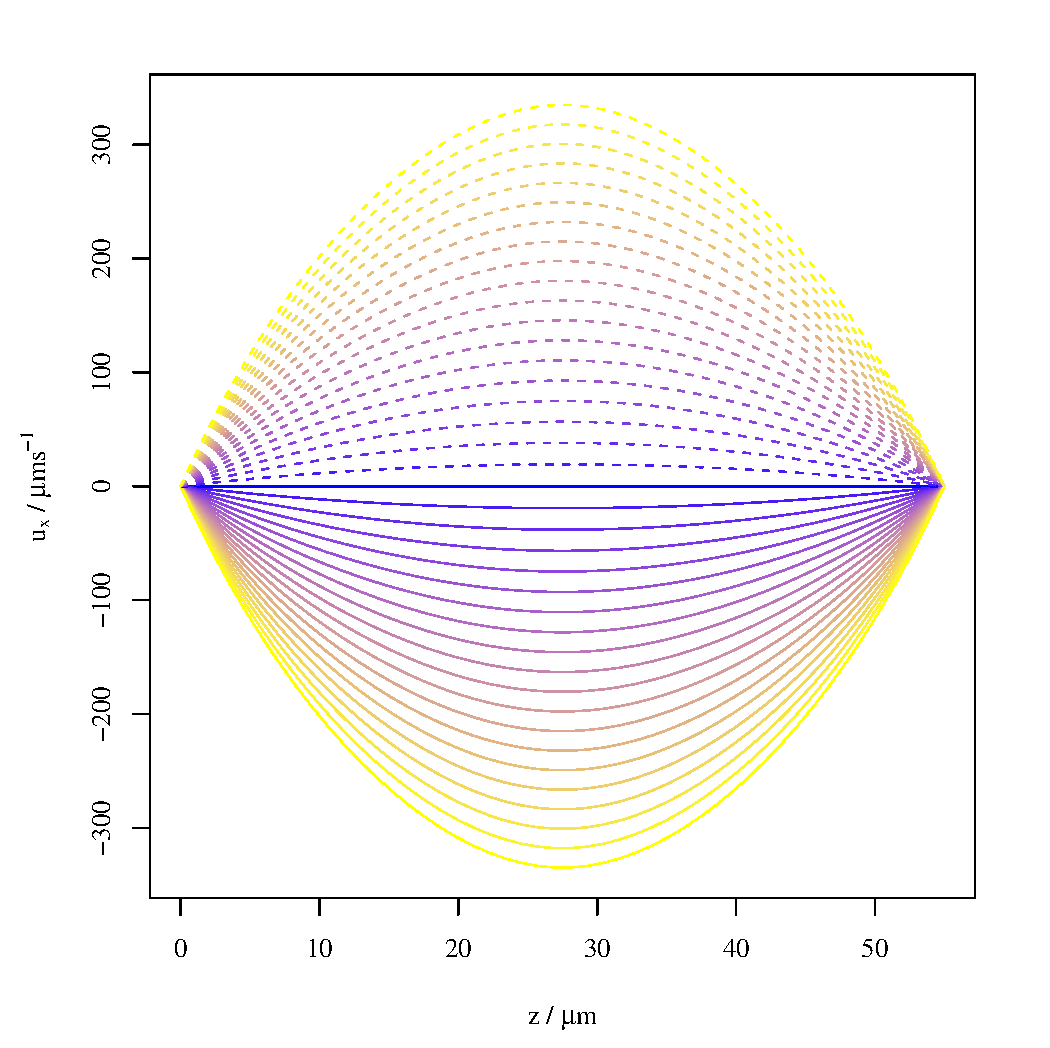
\includegraphics[width=0.49\textwidth]{Figures/diode/model/planar_velocity}}
\subfigure[Flow rates]{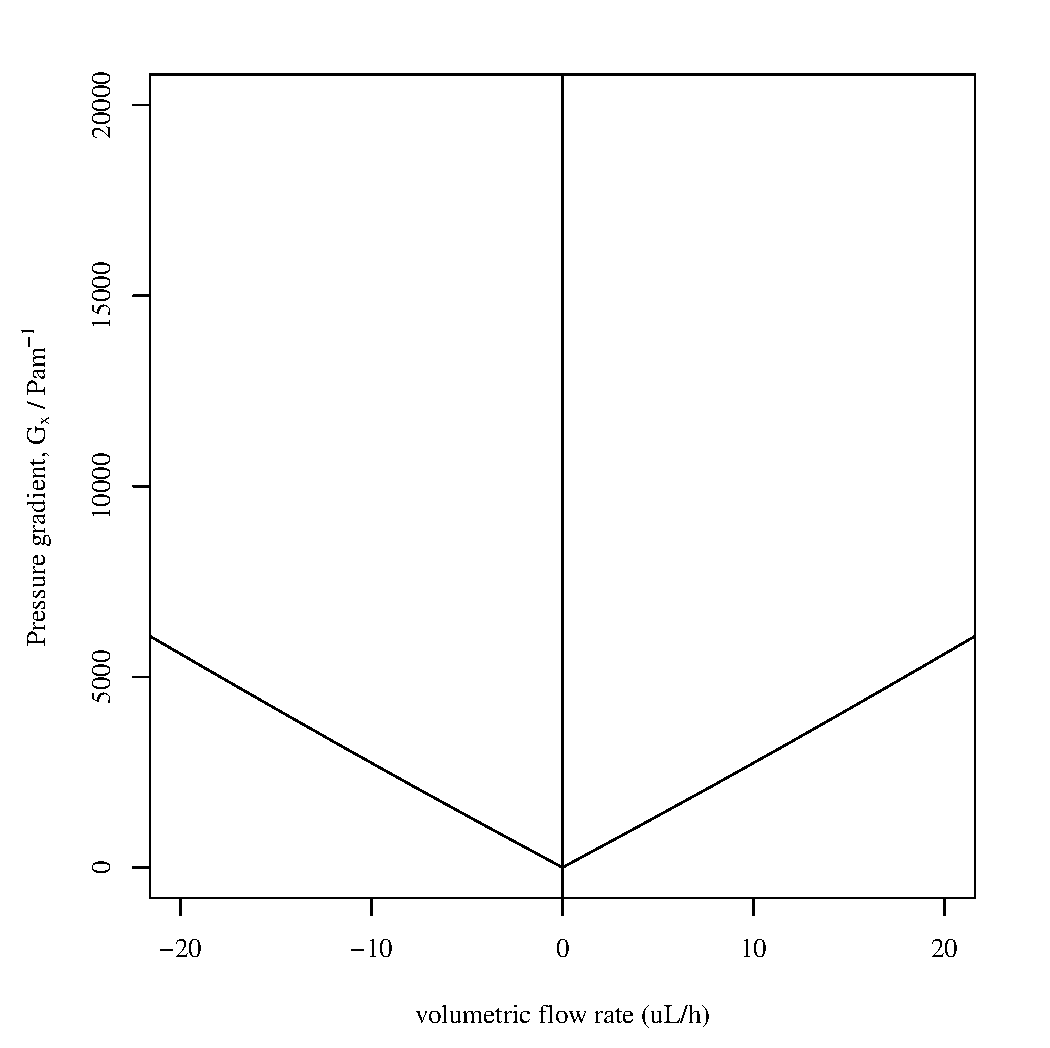
\includegraphics[width=0.49\textwidth]{Figures/diode/model/planar_flow1}}
\end{center}
\caption[Simulated tilt, velocity and pressure gradients for a planar cell]{\label{fig:diode_planar}Planar cell simulation with director profiles ranging from blue (no flow) to yellow (maximum flow). (a) Shows the director tilt profile as a function of volumetric flow rate and flow direction (dashed lines depict positive flow (in the `easy' direction if the system were splayed) and solid lines depict negative flow (in the `hard' direction if the system were splayed)). (b) Velocity profiles in the cell, dashed lines are for flow in the `easy' direction and solid lines are for flow in the `hard' direction. (c) A plot of the simulated volumetric flow rate obtained for the pressure gradient prescribed.}
\end{figure}

\subsection{Vertical}
Figure \ref{fig:diode_homo} shows similar graphs to those shown above in Figure \ref{fig:diode_planar} but here the simulation is made for a cell  within which the director is aligned vertically.

Figure \ref{fig:diode_homo} (a) shows the director tilt profile as a function of flow rate and flow direction. In the positive, or `easy' flow direction (dashed lines), it is seen that the director rotates into the flow in both the top and bottom halves of the cell, becoming more planar, whilst always remaining vertically aligned at the cell mid-plane. This effect has been discussed previously in Chapter \ref{cha:45} where work by Jewell \cite{Jewell2009} showed a nucleated transition between the V-state (director vertical at the cell mid-plane) and the H-state (director horizontal at the cell mid-plane). This transition is not seen in the simulation but is known to exist in experiment. It is also shown in Figure \ref{fig:diode_homo} (a) that for flow in the `hard' direction (solid lines), the same response is observed (as is expected for a cell where the director is aligned vertically). Figure \ref{fig:diode_homo} (b) shows the associated velocity profiles for these distortions (again, identical for flow in both directions, as expected). Figure \ref{fig:diode_homo} (c) shows the associated simulated pressure gradient as a function of the volumetric flow rate through the cell. As expected, there is no difference in the pressure gradient required to achieve a specific volumetric flow rate in either direction. However, there is a non-linear response which can be explained by the large change in director orientation from vertical to near planar at the lower pressure gradients. Once the majority of the cell has switched to the planar state (H-State), a linear form is recovered. Again, Figure \ref{fig:diode_homo} shows, much like Figure \ref{fig:diode_planar}, that for initial director profiles where there is no asymmetry about the $y-z$ plane, there is no difference in the pressure gradient needed to achieve a specific volumetric flow rate. This is of course completely intuitive. In a similar manner to an isotropic fluid, why would one expect any difference between the pressure gradient needed to cause a specific flow rate when flowing a purely planar or purely vertically aligned nematic liquid crystal in either direction? In the next section, simulation regarding a splayed director alignment will be considered.

\begin{figure}
\begin{center}
\subfigure[Tilt profile]{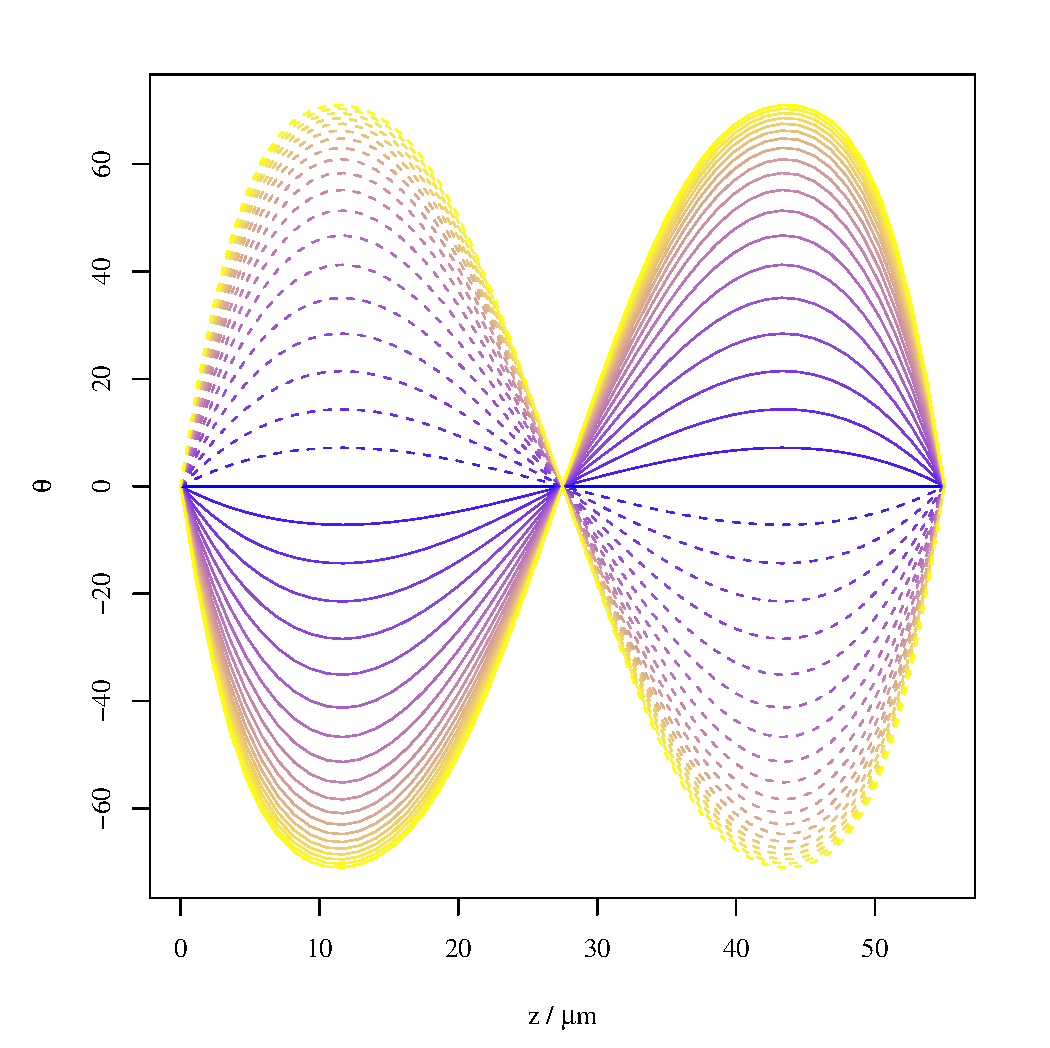
\includegraphics[width=0.49\textwidth]{Figures/diode/model/homo_tilt}}
\subfigure[Velocity profile]{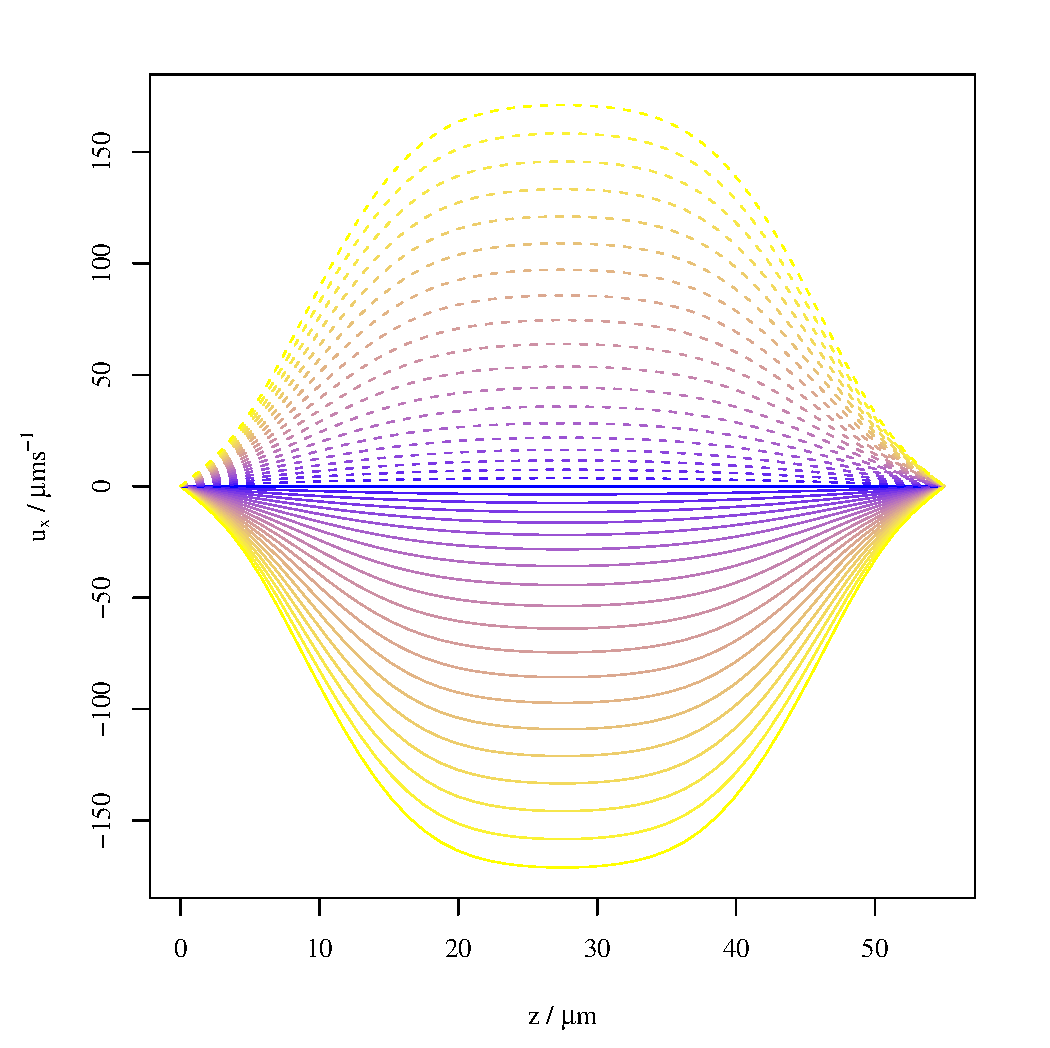
\includegraphics[width=0.49\textwidth]{Figures/diode/model/homo_velocity}}
\subfigure[Flow rates]{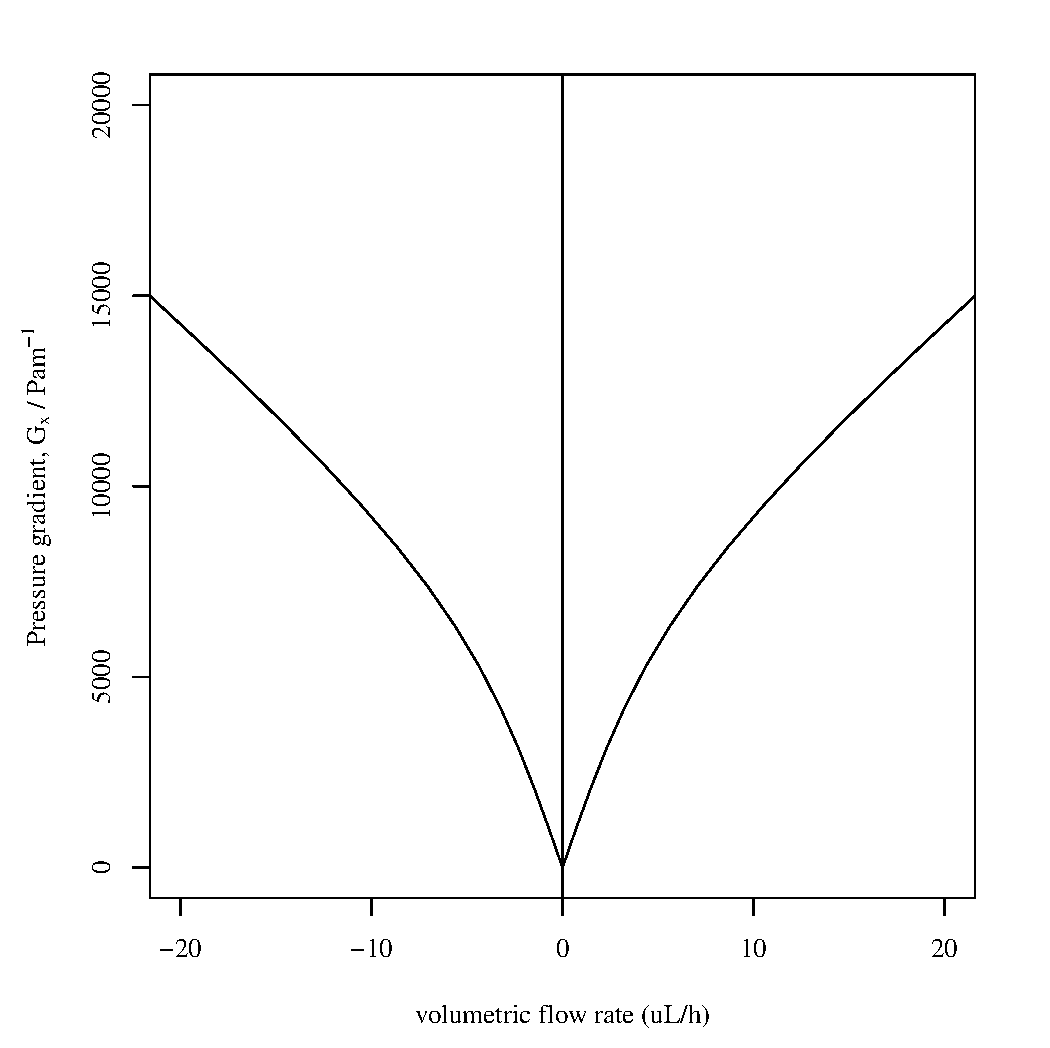
\includegraphics[width=0.49\textwidth]{Figures/diode/model/homo_flow1}}
\end{center}
\caption[Simulated tilt, velocity and pressure gradients for a vertically aligned cell]{\label{fig:diode_homo}Vertically aligned cell simulation with director profiles ranging from blue (no flow) to yellow (maximum flow). (a) Shows the director tilt profile as a function of volumetric flow rate and flow direction (dashed lines depict positive flow (in the `easy' direction if the system were splayed) and solid lines depict negative flow (in the `hard' direction if the system were splayed)). (b) Velocity profiles in the cell, dashed lines are for flow in the `easy' direction and solid lines are for flow in the `hard' direction. (c) A plot of the simulated volumetric flow rate obtained for the pressure gradient prescribed.}
\end{figure}

\subsection{Splayed}
Figure \ref{fig:diode_tilt} again shows (a) the director tilt profiles as a function of volumetric flow rate and flow direction, (b) the velocity profiles as a function of volumetric flow rate and flow direction and (c) the pressure gradient as a function of the volumetric flow rate for a flow cell whereby the director is initially aligned in a splay (maintained horizontal at the cell mid-plane). For these figures as before, the dashed lines represent flow in the `easy' direction, and the solid lines represent flow in the `hard' direction.

\begin{figure}
\begin{center}
\subfigure[Tilt profile]{\includegraphics[width=0.49\textwidth]{Figures/diode/model/tilt_tilt}}
\subfigure[Velocity profile]{\includegraphics[width=0.49\textwidth]{Figures/diode/model/tilt_velocity}}
\subfigure[Flow rates]{\includegraphics[width=0.49\textwidth]{Figures/diode/model/tilt_flow1}}
\end{center}
\caption[Simulated tilt, velocity and pressure gradients for a tilted splayed cell]{\label{fig:diode_tilt} Splayed diode cell simulation with director profiles ranging from blue (no flow) to yellow (maximum flow). (a) Shows the director tilt profile as a function of volumetric flow rate and flow direction (dashed lines depict positive flow (in the `easy' direction) and solid lines depict negative flow (in the `hard' direction)). (b) Velocity profiles in the cell, dashed lines are for flow in the `easy' direction and solid lines are for flow in the `hard' direction. (c) A plot of the simulated volumetric flow rate obtained for the pressure gradient prescribed. }
\end{figure}

Immediately, an interesting response is observed. Figure \ref{fig:diode_tilt} (a) shows that for flow in the `easy' direction, the director  rotates away from the initially tilted alignment condition at the cell boundary, towards the Leslie angle in the top and bottom quarters of the cell. This is seen in the flattening of the dashed curves at values of $\pm11^{\circ}$ away from $90^{\circ}$ in both halves of the cell. It is clear that the director is saturating at the Leslie angle (of opposite sign) in both the top and bottom halves of the cell (as also shown in Figure \ref{fig:diode_planar}). When the flow is simulated for the `hard' direction against the splay (solid lines in Figure \ref{fig:diode_tilt} (a)) a completely different director profile is observed. Now it is seen that the director initially rotates backwards almost $100^{\circ}$, through vertical alignment, to come towards planar alignment in the bottom quarter of the cell. The director then rotates rapidly back through planar alignment at the cell mid-plane, before repeating the large rotation through vertical alignment in the top half of the cell and finally returning to the initial tilted angle at the cell boundary. This is clearly a very complicated distortion whereby the director `backbends' on itself twice. This results in four regions of the cell where the director rotates through a vertical position \footnote{Of course, much like the V and H-State reported by Jewell \cite{Jewell2009}, it is likely that this system will undergo a nucleated transition to a more energetically favourable director profile.}. The associated simulated velocity profiles shown in Figure \ref{fig:diode_tilt} (b) confirm that the velocities achieved for a given pressure gradient in the `easy' direction (dashed lines) are much higher than those achieved for the same pressure gradient in the `hard' flow direction. This can of course be attributed to the large distortion occurring in the director profile when flowing in the `hard' direction.
Figure \ref{fig:diode_tilt} (c) perhaps most strikingly shows the difference in the pressure gradient required for the same volumetric flow rate when flown in the `easy' and `hard' directions. Here it can be seen that for a volumetric flow rate of $20 \mu L/h$ in the easy direction (positive flow rates) a pressure gradient of 10000 Pa m$^{-1}$ is required. For the same volumetric flow rate in the hard direction, a pressure gradient of almost 20000 Pa m$^{-1}$ is required.



\subsection{Data and simulation}
Figure \ref{fig:simulation_data} shows a plot of the simulated pressure gradient compared to the data obtained from the experiments described in Section \ref{sec:second_diode}. Here, the data from Section \ref{sec:second_diode} (originally shown as differences in the column height measured in mm) has been converted to a pressure gradient across the length of the cell using equation \ref{eq:pressures} and dividing the result by the distance between the two manometer tubes on the cell to give Pa/m.\footnote{Values of $g=9.8$ m/s$^2$ and $\rho=1020$ kg/m$^3$ from Stewart \cite{Stewart2004} were used.} 

Figure \ref{fig:simulation_data} (a) shows the data from Figure \ref{fig:iso_diode_diff} presented as a function of volumetric flow rate, where flow against the splay, or in the `hard' direction, is plotted with negative flow rates. The simulated response is calculated for flow in a cell that has an initial splayed director profile tilted at an angle of $50^{\circ}$ away from the surface (going through planar at $z=d/2$). It is seen that for flow in the `easy' direction (positive flow rates), fairly good agreement is seen between the model and data, with a linear correlation between the flow rate and the pressure gradient measured across the cell. At low flow rates, the small non linearity in the data does not appear to agree with the simulation, although as stated earlier, this response may be due to a calibration error when changing over to the smaller syringe. Certainly, one would expect the pressure gradient to have a value of 0 Pa/m when the flow rate is 0 $\mu$ L/h. In general, the magnitude of the measured pressure gradient as  function of the volumetric flow appears to agree with the data from the experiment. For flow in the `hard' direction, good agreement between the model and data is shown with a clear non linear correlation between the volumetric flow rate and the pressure gradient across the cell. For flow in the `hard' direction,  a steep increase in the pressure gradient is shown at low flow rates, before becoming less steep at higher flow rates. Again, the magnitude of the measured pressure gradient as function of the volumetric flow appears to agree with the data from the experiment, with the added agreement of the non linear shape to the response.

\begin{figure}
\begin{center}
\subfigure[Data and simulation]{\includegraphics[width=0.6\textwidth]{Figures/Diode/simulation_new_modeldata}}
\subfigure[Simulated tilt profile]{\includegraphics[width=0.6\textwidth]{Figures/Diode/simulation_new_tilt}}
\end{center}
\caption[Comparison of experimental and simulated pressure gradients as a function of flow rate and direction]{\label{fig:simulation_data}(a) Shows the simulated pressure gradient as a function of the volumetric flow rate (red lines) and the data obtained from experiment (circles). The cell is simulated to have a tilt angle of 50$^{\circ}$ (measured from the surface) in a splayed geometry. (b) The simulated director tilt profile for the simulates curves shown in (a). Again, dashed lines depict positive flow (in the `easy' direction) and solid lines depict negative flow (in the `hard' direction). Much like as is seen in Figure \ref{fig:diode_tilt} (a), the director is seen to achieve the Leslie angle for flow in the positive direction, whilst performing a complex back bended profile for flow in the negative direction.}
\end{figure}

The dramatic reorientation of the director for flow in the `hard' direction is shown in the simulated director profile of Figure \ref{fig:simulation_data} (b) which show a very similar response to the simulated curves first shown in Figure \ref{fig:diode_tilt} (a) for a splayed geometry of $45^{\circ}$. Here, Figure \ref{fig:simulation_data} (b) shows that for flow in the `hard' direction (solid lines), the director rotates back upon itself from its initial alignment, going through vertical orientation at four points within the cell. As a function of the cell depth, beginning at $z=0$, the director rotates backwards through $0^{\circ}$ (vertical) to a tilt angle of approximately $-60^{\circ}$ at $z=d/5$, before rotating in the opposite direction, back through $0^{\circ}$ to become planar $90^{\circ}$ at the cell mid-plane $\left(z=d/2\right)$. In the top half of the cell, the director completes the same orientation as a function of cell depth, with the director going through vertical alignment again at two points in $z$ before coming to its initial alignment angle at $z=d$. For flow in the `easy' direction (dashed lines), the director is seen to come to the Leslie angle of opposite sign in the top and bottom halves of the cell, always remaining planar at the cell mid-plane.

Figure \ref{fig:simulation_iso} also shows a plot of the data taken from Section \ref{sec:iso_experiment} Figure \ref{fig:iso_diode_diff}, for flow during the isotropic phase. Here it is clear that the asymmetry between flow in the positive and negative direction (which is shown previously for the liquid crystalline phase in Figure \ref{fig:simulation_data} (a)) is no longer present. Along with the now symmetric response for flow in both directions, the overall pressure gradient across the cell has dramatically decreased. Here, a plot of the simulated pressure gradient for a planar aligned cell has been included (red lines), showing a fairly good fit in terms of response and magnitude.

\begin{figure}
\begin{center}
\includegraphics[width=0.6\textwidth]{Figures/Diode/simulation_new_iso}
\end{center}
\caption[Comparison of experimental data and simulation for flow in the isotropic phase]{\label{fig:simulation_iso}Here the pressure gradient as a function of volumetric flow rate is plotted for flow in the isotropic phase. The simulated response is also plotted (red lines) for  flow in a cell where the director is aligned planar homogeneously, as shown in Figure \ref{fig:diode_planar}.}
\end{figure}

A further schematic representation of the director distortion in both the `easy' and `hard' directions is given in Figure \ref{fig:easy_hard}. Here the flow in the `easy' direction is shown by the green arrow, whereby the director rotates to achieve the Leslie angle in the top and bottom halves of the cell. For flow in the `hard' direction (red arrow) the complex back-bending is depicted.

\begin{figure}
\begin{center}
\includegraphics[width=0.5\textwidth]{Figures/Diode/easy_hard}
\end{center}
\caption[Schematic diagram of the simulated director profiles for flow in the `easy' and `hard' directions]{\label{fig:easy_hard}A schematic diagram depicting the simulated director distortion for flow in the `easy' direction (green arrow) whereby the director achieves the Leslie angle in the majority of the cell. In the `hard' direction (red arrow), the director back bends upon itself to create a highly distorted director profile. Although not shown in this figure due to space, under flow in the `hard' direction, the director goes through vertical alignment at four points in $z$.}
\end{figure}

\section{Conclusions}
In this chapter it has been experimentally shown that there may be a difference in the pressure gradient required to achieve the same volumetric flow rate through a cell that contains a nematic liquid crystal in a splayed geometry aligned azimuthally parallel to the flow direction. As such, it suggests that under the right conditions, there can exist some diode or `valve-like' behaviour from the alignment of the liquid crystal itself.

It has been shown that for cells given the correct initial alignment conditions, a difference in the pressure gradient measured across the cell can be observed when prescribing the same volumetric rate to flow in opposite directions. From these experiments it can be seen that for flow in the `easy' direction, an almost linear relationship is observed between the volumetric flow rate and the pressure gradient, with the director simulated to achieve the Leslie angle of opposite sign in the top bottom halves of the cell. For flow in the `hard' direction, a non-linear response is seen in the pressure gradient as a function of the volumetric flow rate. For all flow rates, the pressure gradient required is larger for flow in the `hard' direction than for flow in the `easy' direction. Both responses also show fairly good agreement with the results from simulation.

As the system is heated to the isotropic phase, the magnitude of the pressure gradient is seen to reduce (as expected for a system of lowered viscosity) and the difference in these pressure gradients for flow in both directions has also decreased, \textit{but has critically not gone to zero in every case}. The response of the pressure gradient as a function of the volumetric flow rate is also shown to be very similar to that simulated for a cell that is initially aligned planar homogeneously.

Some thoughts on experimental and procedural improvements to this experiment. The method of data abstraction presented in this chapter is physically difficult and prone to human error. A primary cause of concern is the rectangular cross-sectional flow channels, which are used because they allow for relatively easy production of the desired director profile by treatment of the aligning surfaces. If by some method, one were able to produce these splayed director profiles in a fine capillary or circular cross-sectioned flow channel (director dynamics in capillaries has previously been a topic of interest \cite{Cladis1972,Palffy-muhoray1993,Ziherl1996}), the ability for any azimuthal rotation of the director would be removed by the symmetry of the channel. As such, some very preliminary simulation has been tested for this study, examining flow in a capillary \cite{Athertona}, with early results suggesting that a similar director response is observed, where for flow in the `easy' direction the director quickly achieves the Leslie angle and for flow in the `hard' direction a complex back bending of the director is observed. Of course, with such a capillary flow channel, measuring the pressure gradient is also likely to be made a more difficult task due to the the size of the capillary and the geometry of the curved glass surfaces\footnote{Some preliminary experiments into creating circular cross-sectional flow channels have also been made as part of this study. This has involved the setting of electrical wire in Polydimethylsiloxane (PDMS) (a silicon based organic polymer) and drawing it out to leave a smooth flow channel behind. A common problem here is that the PDMS does not always cure hard and can expand and contract when pressure is applied.}. If one wanted to image or probe the director's response simultaneously with flow, this is also likely to be more difficult.

Finally, for this experiment it is advisable to reduce the number of connections and tubes to the minimum necessary. The experiments described in this chapter have a total of eleven connections (six at the valve, four at the cell and one at the syringe). It is indeed very difficult to ensure that all of these connections are secure and not leaking (particularly when the cell is in the closed polystyrene housing for the isotropic-phase experiment).
